\documentclass[]{article}
\usepackage{lmodern}
\usepackage{amssymb,amsmath}
\usepackage{ifxetex,ifluatex}
\usepackage{fixltx2e} % provides \textsubscript
\ifnum 0\ifxetex 1\fi\ifluatex 1\fi=0 % if pdftex
  \usepackage[T1]{fontenc}
  \usepackage[utf8]{inputenc}
\else % if luatex or xelatex
  \ifxetex
    \usepackage{mathspec}
  \else
    \usepackage{fontspec}
  \fi
  \defaultfontfeatures{Ligatures=TeX,Scale=MatchLowercase}
\fi
% use upquote if available, for straight quotes in verbatim environments
\IfFileExists{upquote.sty}{\usepackage{upquote}}{}
% use microtype if available
\IfFileExists{microtype.sty}{%
\usepackage{microtype}
\UseMicrotypeSet[protrusion]{basicmath} % disable protrusion for tt fonts
}{}
\usepackage[margin=1in]{geometry}
\usepackage{hyperref}
\hypersetup{unicode=true,
            pdftitle={Laborator 6},
            pdfborder={0 0 0},
            breaklinks=true}
\urlstyle{same}  % don't use monospace font for urls
\usepackage{natbib}
\bibliographystyle{plainnat}
\usepackage{color}
\usepackage{fancyvrb}
\newcommand{\VerbBar}{|}
\newcommand{\VERB}{\Verb[commandchars=\\\{\}]}
\DefineVerbatimEnvironment{Highlighting}{Verbatim}{commandchars=\\\{\}}
% Add ',fontsize=\small' for more characters per line
\usepackage{framed}
\definecolor{shadecolor}{RGB}{248,248,248}
\newenvironment{Shaded}{\begin{snugshade}}{\end{snugshade}}
\newcommand{\KeywordTok}[1]{\textcolor[rgb]{0.13,0.29,0.53}{\textbf{#1}}}
\newcommand{\DataTypeTok}[1]{\textcolor[rgb]{0.13,0.29,0.53}{#1}}
\newcommand{\DecValTok}[1]{\textcolor[rgb]{0.00,0.00,0.81}{#1}}
\newcommand{\BaseNTok}[1]{\textcolor[rgb]{0.00,0.00,0.81}{#1}}
\newcommand{\FloatTok}[1]{\textcolor[rgb]{0.00,0.00,0.81}{#1}}
\newcommand{\ConstantTok}[1]{\textcolor[rgb]{0.00,0.00,0.00}{#1}}
\newcommand{\CharTok}[1]{\textcolor[rgb]{0.31,0.60,0.02}{#1}}
\newcommand{\SpecialCharTok}[1]{\textcolor[rgb]{0.00,0.00,0.00}{#1}}
\newcommand{\StringTok}[1]{\textcolor[rgb]{0.31,0.60,0.02}{#1}}
\newcommand{\VerbatimStringTok}[1]{\textcolor[rgb]{0.31,0.60,0.02}{#1}}
\newcommand{\SpecialStringTok}[1]{\textcolor[rgb]{0.31,0.60,0.02}{#1}}
\newcommand{\ImportTok}[1]{#1}
\newcommand{\CommentTok}[1]{\textcolor[rgb]{0.56,0.35,0.01}{\textit{#1}}}
\newcommand{\DocumentationTok}[1]{\textcolor[rgb]{0.56,0.35,0.01}{\textbf{\textit{#1}}}}
\newcommand{\AnnotationTok}[1]{\textcolor[rgb]{0.56,0.35,0.01}{\textbf{\textit{#1}}}}
\newcommand{\CommentVarTok}[1]{\textcolor[rgb]{0.56,0.35,0.01}{\textbf{\textit{#1}}}}
\newcommand{\OtherTok}[1]{\textcolor[rgb]{0.56,0.35,0.01}{#1}}
\newcommand{\FunctionTok}[1]{\textcolor[rgb]{0.00,0.00,0.00}{#1}}
\newcommand{\VariableTok}[1]{\textcolor[rgb]{0.00,0.00,0.00}{#1}}
\newcommand{\ControlFlowTok}[1]{\textcolor[rgb]{0.13,0.29,0.53}{\textbf{#1}}}
\newcommand{\OperatorTok}[1]{\textcolor[rgb]{0.81,0.36,0.00}{\textbf{#1}}}
\newcommand{\BuiltInTok}[1]{#1}
\newcommand{\ExtensionTok}[1]{#1}
\newcommand{\PreprocessorTok}[1]{\textcolor[rgb]{0.56,0.35,0.01}{\textit{#1}}}
\newcommand{\AttributeTok}[1]{\textcolor[rgb]{0.77,0.63,0.00}{#1}}
\newcommand{\RegionMarkerTok}[1]{#1}
\newcommand{\InformationTok}[1]{\textcolor[rgb]{0.56,0.35,0.01}{\textbf{\textit{#1}}}}
\newcommand{\WarningTok}[1]{\textcolor[rgb]{0.56,0.35,0.01}{\textbf{\textit{#1}}}}
\newcommand{\AlertTok}[1]{\textcolor[rgb]{0.94,0.16,0.16}{#1}}
\newcommand{\ErrorTok}[1]{\textcolor[rgb]{0.64,0.00,0.00}{\textbf{#1}}}
\newcommand{\NormalTok}[1]{#1}
\usepackage{longtable,booktabs}
\usepackage{graphicx,grffile}
\makeatletter
\def\maxwidth{\ifdim\Gin@nat@width>\linewidth\linewidth\else\Gin@nat@width\fi}
\def\maxheight{\ifdim\Gin@nat@height>\textheight\textheight\else\Gin@nat@height\fi}
\makeatother
% Scale images if necessary, so that they will not overflow the page
% margins by default, and it is still possible to overwrite the defaults
% using explicit options in \includegraphics[width, height, ...]{}
\setkeys{Gin}{width=\maxwidth,height=\maxheight,keepaspectratio}
\IfFileExists{parskip.sty}{%
\usepackage{parskip}
}{% else
\setlength{\parindent}{0pt}
\setlength{\parskip}{6pt plus 2pt minus 1pt}
}
\setlength{\emergencystretch}{3em}  % prevent overfull lines
\providecommand{\tightlist}{%
  \setlength{\itemsep}{0pt}\setlength{\parskip}{0pt}}
\setcounter{secnumdepth}{5}
% Redefines (sub)paragraphs to behave more like sections
\ifx\paragraph\undefined\else
\let\oldparagraph\paragraph
\renewcommand{\paragraph}[1]{\oldparagraph{#1}\mbox{}}
\fi
\ifx\subparagraph\undefined\else
\let\oldsubparagraph\subparagraph
\renewcommand{\subparagraph}[1]{\oldsubparagraph{#1}\mbox{}}
\fi

%%% Use protect on footnotes to avoid problems with footnotes in titles
\let\rmarkdownfootnote\footnote%
\def\footnote{\protect\rmarkdownfootnote}

%%% Change title format to be more compact
\usepackage{titling}

% Create subtitle command for use in maketitle
\newcommand{\subtitle}[1]{
  \posttitle{
    \begin{center}\large#1\end{center}
    }
}

\setlength{\droptitle}{-2em}
  \title{Laborator 6}
  \pretitle{\vspace{\droptitle}\centering\huge}
  \posttitle{\par}
\subtitle{Regresie liniară simplă și multiplă}
  \author{}
  \preauthor{}\postauthor{}
  \date{}
  \predate{}\postdate{}

\usepackage{booktabs}
\usepackage{longtable}
\usepackage{framed,color}
\definecolor{shadecolor}{RGB}{248, 248, 248}
%\definecolor{shadecolor1}{RGB}{216,225,235}
%\definecolor{framecolor}{RGB}{108,123,13}

%\definecolor{shadecolor}{RGB}{226, 255, 241}
\definecolor{shadecolor1}{RGB}{217,225,199}
\definecolor{framecolor}{RGB}{60,179,113}

\ifxetex
  \usepackage{letltxmacro}
  \setlength{\XeTeXLinkMargin}{1pt}
  \LetLtxMacro\SavedIncludeGraphics\includegraphics
  \def\includegraphics#1#{% #1 catches optional stuff (star/opt. arg.)
    \IncludeGraphicsAux{#1}%
  }%
  \newcommand*{\IncludeGraphicsAux}[2]{%
    \XeTeXLinkBox{%
      \SavedIncludeGraphics#1{#2}%
    }%
  }%
\fi

\newenvironment{frshaded*}{%
  \def\FrameCommand{\fboxrule=\FrameRule\fboxsep=\FrameSep \fcolorbox{framecolor}{shadecolor1}}%
  \MakeFramed {\advance\hsize-\width \FrameRestore}}%
{\endMakeFramed}

\newenvironment{rmdblock}[1]
  {\begin{frshaded*}
  \begin{itemize}
  \renewcommand{\labelitemi}{
    \raisebox{-.7\height}[0pt][0pt]{
      {\setkeys{Gin}{width=2em,keepaspectratio}\includegraphics{images/icons/#1}}
    }
  }
  \item
  }
  {
  \end{itemize}
  \end{frshaded*}
  }

\newenvironment{rmdcaution}
  {\begin{rmdblock}{caution}}
  {\end{rmdblock}}
% \newenvironment{rmdinsight}
%   {\begin{rmdblock}{insight}}
%   {\end{rmdblock}}
\newenvironment{rmdexercise}
  {\begin{rmdblock}{exercise}}
  {\end{rmdblock}}
\newenvironment{rmdtip}
  {\begin{rmdblock}{tip}}
  {\end{rmdblock}}

%%%%%%%%%%%%%%%%%%%%%%%%%%%%%%%%%%%%%%%%%%%%%%%%%%%%%%%%%
%\usepackage{hyperref}
%\hypersetup{unicode=true,
%            pdftitle={Curs Biostatistica 2018},
%            pdfauthor={Alexandru Amarioarei},
%            pdfborder={0 0 0},
%            colorlinks,%
%            citecolor=green,%
%            filecolor=green,%
%            linkcolor=green,%
%            urlcolor=green}
%\urlstyle{same}

%%%%%%%%%%%%%%%%%%%%%%%%%%%%%%%%%%%%%%%%%%%%%%%%%%%%%%%%%%%%%%%%%%%%%%%%%%%%%%%%%%%%%%%%%%%%%%%%%%%%%%%%%%%%%%%%%%%%%
%%%%%%%%%%% For insight block %%%%%%%%%%%%%%%%%%%%%%%%%%
\definecolor{shadecolor_insight}{RGB}{223,240,216}
\definecolor{framecolor_insight}{RGB}{136,193,137}

%\definecolor{shadecolor_insight}{RGB}{217,225,199}
%\definecolor{framecolor_insight}{RGB}{60,179,113}

\newenvironment{frshaded_insight*}{%
  \def\FrameCommand{\fboxrule=\FrameRule\fboxsep=\FrameSep \fcolorbox{framecolor_insight}{shadecolor_insight}}%
  \MakeFramed {\advance\hsize-\width \FrameRestore}}%
{\endMakeFramed}

\newenvironment{rmdblock_insight}[1]
  {\begin{frshaded_insight*}
  \begin{itemize}
  \renewcommand{\labelitemi}{
    \raisebox{-.7\height}[0pt][0pt]{
      {\setkeys{Gin}{width=2em,keepaspectratio}\includegraphics{images/icons/#1}}
    }
  }
  \item
  }
  {
  \end{itemize}
  \end{frshaded_insight*}
  }

\newenvironment{rmdinsight}
  {\begin{rmdblock_insight}{insight}}
  {\end{rmdblock_insight}}

%%%%%%%%%%%%%%%%%%%%%%%%%%%%%%%%%%%%%%%%%%%%%%%%%%%%%%%%%%%%%%%%%%%%%%%%%%%%%%%%%%%%%%%%%%%%%%%%%%%%%%%%%%%%%%%%%%%%%
\usepackage{subfigure}
\usepackage{booktabs}
\usepackage{slashbox}
\usepackage{color}
%%%%%%%%%%%%%%%%%%%%%%%%%%%%%%%%%%%%%%%%%
\definecolor{linkcol}{rgb}{0,0,0.4}
\definecolor{citecol}{rgb}{0.5,0,0}

% Change this to change the informations included in the pdf file
% \usepackage[pagebackref]{hyperref}
% \usepackage[verbose]{backref}
% \backrefsetup{verbose=false}
\usepackage[hyperpageref]{backref}
% \PassOptionsToPackage{pagebackref}{hyperref}
% See hyperref documentation for information on those parameters

\hypersetup
{
bookmarksopen=true,
pdftitle="Curs Biostatistica",
pdfauthor="Alexandru Amarioarei",
pdfsubject="Laboratoare Biostatistica", %subject of the document
pdfmenubar=true, %menubar shown
pdfhighlight=/O, %effect of clicking on a link
colorlinks=true, %couleurs sur les liens hypertextes
pdfpagemode=None, %aucun mode de page
pdfpagelayout=SinglePage, %ouverture en simple page
pdffitwindow=true, %pages ouvertes entierement dans toute la fenetre
linkcolor=linkcol, %couleur des liens hypertextes internes
citecolor=citecol, %couleur des liens pour les citations
urlcolor=linkcol %couleur des liens pour les url
}


% set the back references
\renewcommand*{\backref}[1]{}
\renewcommand*{\backreftwosep}{ și~} % inserted between entries 
                              % in a list of two entries, 
                              % default is " and~".
\renewcommand*{\backreflastsep}{, și~} % inserted between the last 
                               % two entries of a list with more
                               % than two entries, default is ", and~".
\renewcommand*{\backrefalt}[4]{%
    \ifcase #1 (Necitat.)%
    \or        (Citat la pagina~#2.)%
    \else      (Citat la paginile~#2.)%
    \fi}


%%%%%%%%%%%%%%%%%%%%%%%%%%%%%%%%%%%%%%%%%%%%%%%%%%%%%%%%%%%%%%%%%%%%%%%%%%%%%%%%%%%%%%%%%%%%%%%%%%%%%%%%%%%%%%%%%%%%%
%CITEVA DEFINITII
\def\om{\omega}
\def\Om{\Omega}
\def\et{\eta}
\def\td{\tilde{\delta}}
\def\m{{\mu}}
\def\n{{\nu}}
\def\k{{\kappa}}
\def\l{{\lambda}}
\def\L{{\Lambda}}
\def\g{{\gamma}}
\def\a{{\alpha}}
\def\e{{\varepsilon}}
\def\b{{\beta}}
\def\G{{\Gamma}}
\def\d{{\delta}}
\def\D{{\Delta}}
\def\t{{\theta}}
\def\s{{\sigma}}
\def\S{{\Sigma}}
\def\z{{\zeta}}
\def\qed{\hfill\Box}
\def\ds{\displaystyle}
\def\mc{\mathcal}
%%%%%%%%%%%%%%%%%%%%%%%%%%%%%%%%%%%%%%%%%%%%%%%%%%%%%%%%%%%%%%%%%%%%%%%%%%%%%%%%%%%%%%%%%%%%%%%%%%%%%%%%%%%%%%%%%%%%%%
\def\1{{\mathbf 1}}
\def\CC{{\mathbb C}}
\def\VV{{\mathbb V}}
\def\RR{{\mathbb R}}
\def\QQ{{\mathbb Q}}
\def\ZZ{{\mathbb Z}}
\def\PP{{\mathbb P}}
\def\EE{{\mathbb E}}
\def\NN{{\mathbb N}}
\def\FF{{\mathbb F}}
%\def\SS{{\mathbb S}}
\def\MA{{\mathcal A}}
\def\MO{{\mathcal O}}
\def\MF{{\mathcal F}}
\def\ME{{\mathcal E}}
\def\MR{{\mathcal R}}
\def\MB{{\mathcal B}}
\def\MM{{\mathcal M}}
\def\MN{{\mathcal N}}
\def\MU{{\mathcal U}}
\def\MP{{\mathcal P}}
\def\MS{{\mathcal S}}
\def\MBS{{\mathbf S}}
\def\MX{{\bm{ \mathscr X}}}

% independent sign
\newcommand\independent{\protect\mathpalette{\protect\independenT}{\perp}}
\def\independenT#1#2{\mathrel{\rlap{$#1#2$}\mkern2mu{#1#2}}}

\renewcommand\tablename{Tab.}
\renewcommand{\figurename}{Fig.}
\renewcommand\refname{Referințe}

%%%%%%%%%%%%%%%%%%%%%%%%%%%%%%%%%%%%%%%%%%%%%%%%%%%%%%%%%%%%%%%%%%%%%%%%%%%%%%%%%%%%%%%%%%%%%%%%%%%%%%%%%%%%%%%%%%%%%
%Header and Footer
\usepackage{fancyhdr}

\pagestyle{fancy}
\fancyhf{}
\rhead{Universitatea din Bucure\c sti\\ Facultatea de Matematic\u a \c si Informatic\u a}
\lhead{\textit{Curs}: Biostatistic\u a 2018\\ \textit{Instructor}: A. Am\u arioarei}
\rfoot{Pagina \thepage}
\lfoot{Grupa: 503}
%%%%%%%%%%%%%%%%%%%%%%%%%%%%%%%%%%%%%%%
\usepackage{booktabs}
\usepackage{longtable}
\usepackage{array}
\usepackage{multirow}
\usepackage[table]{xcolor}
\usepackage{wrapfig}
\usepackage{float}
\usepackage{colortbl}
\usepackage{pdflscape}
\usepackage{tabu}
\usepackage{threeparttable}
\usepackage{threeparttablex}
\usepackage[normalem]{ulem}
\usepackage{makecell}

\begin{document}
\maketitle

%%%%%%%%%%%%%%%%%%%%%%%%
\thispagestyle{fancy}

Obiectivul acestui laborator este de a prezenta câteva noțiuni legate de
problema de regresie.

\section{Regresie liniară simplă}\label{regresie-liniara-simpla}

Regresia liniară simplă (sau \emph{modelul liniar simplu}) este un
instrument statistic utilizat pentru a descrie relația dintre două
variabile aleatoare, \(X\) (variabilă \emph{cauză}, \emph{predictor} sau
\emph{covariabilă}) și \(Y\) (variabilă \emph{răspuns} sau \emph{efect})
și este definit prin

\[
\mathbb{E}[Y|X=x]=\beta_0+\beta_1x 
\]

sau altfel spus

\[
Y = \beta_0 + \beta_1 X + \varepsilon.
\]

În relațiile de mai sus, \(\beta_0\) și \(\beta_1\) sunt cunoscute ca
ordonata la origine (\emph{intercept}) și respectiv panta (\emph{slope})
dreptei de regresie.

Ipotezele modelului sunt:

\begin{enumerate}
\def\labelenumi{\roman{enumi}.}
\tightlist
\item
  \textbf{Linearitatea}: \(\mathbb{E}[Y|X=x]=\beta_0+\beta_1x\)
\item
  \textbf{Homoscedasticitatea}:
  \(\mathbb{V}\text{ar}(\varepsilon_i)=\sigma^2\), cu \(\sigma^2\)
  constantă pentru \(i=1,\ldots,n\)
\item
  \textbf{Normalitatea}: \(\varepsilon_i\sim\mathcal{N}(0,\sigma^2)\)
  pentru \(i=1,\ldots,n\)
\item
  \textbf{Independența erorilor}: \(\varepsilon_1,\ldots,\varepsilon_n\)
  sunt independente (sau necorelate,
  \(\mathbb{E}[\varepsilon_i\varepsilon_j]=0\), \(i\neq j\), deoarece
  sunt presupuse normale)
\end{enumerate}

Altfel spus

\[
Y|X=x\sim \mathcal{N}(\beta_0+\beta_1x,\sigma^2)
\]

\begin{rmdinsight}
\begin{itemize}
\item
  Nicio ipoteză nu a fost făcută asupra repartiției lui \(X\) (poate fi
  sau deterministă sau aleatoare)
\item
  Modelul de regresie presupune că \textbf{\(Y\) este continuă} datorită
  normalității erorilor. În orice caz, \textbf{\(X\) poate fi o
  variabilă discretă}!
\end{itemize}
\end{rmdinsight}

\begin{center}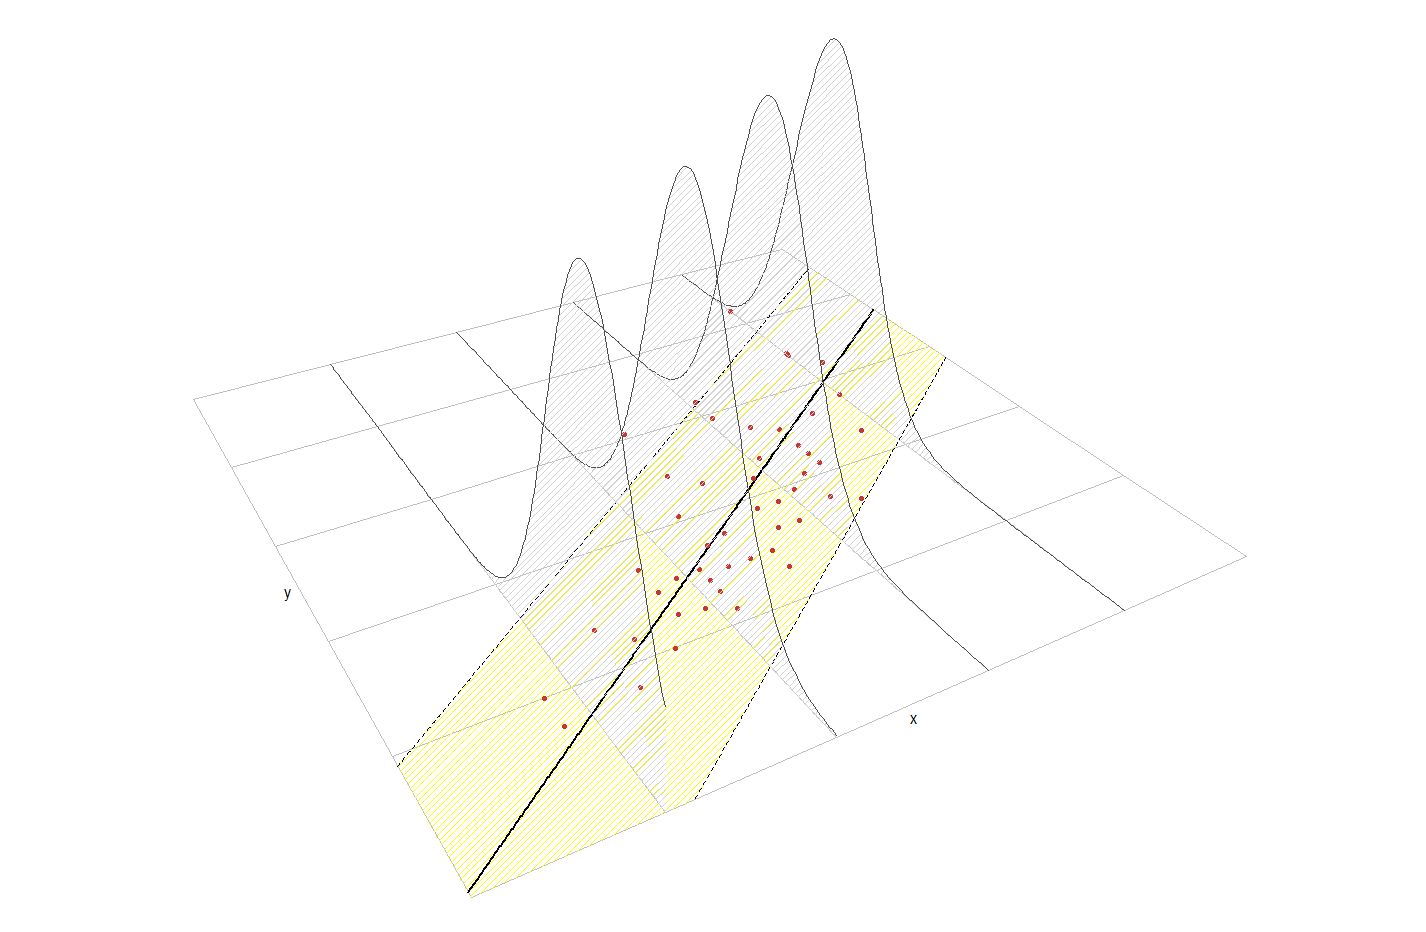
\includegraphics[width=0.8\linewidth]{images/lab6/RegresiaLiniara} \end{center}

Dat fiind un eșantion \((X_1,Y_1),\ldots,(X_n,Y_n)\) pentru variabilele
\(X\) și \(Y\) putem estima coeficienții necunoscuți \(\beta_0\) și
\(\beta_1\) minimizând \emph{suma abaterilor pătratice reziduale}
(\emph{Residual Sum of Squares} - RSS)

\[
\text{RSS}(\beta_0,\beta_1)=\sum_{i=1}^n(Y_i-\beta_0-\beta_1X_i)^2
\]

ceea ce conduce la

\[
\hat\beta_0=\bar{Y}-\hat\beta_1\bar{X},\quad \hat\beta_1=\frac{s_{xy}}{s_{xx}^2}=\frac{\sum_{i=1}^{n}{(X_i-\bar{X})}Y_i}{\sum_{i=1}^{n}{(X_i-\bar{X})^2}}
\]

unde

\begin{itemize}
\tightlist
\item
  \(\bar{X}=\frac{1}{n}\sum_{i=1}^nX_i\) este \emph{media eșantionului}
\item
  \(s_{xx}^2=\frac{1}{n}\sum_{i=1}^n(X_i-\bar{X})^2\) este
  \emph{varianța eșantionului}
\item
  \(s_{xy}=\frac{1}{n}\sum_{i=1}^n(X_i-\bar{X})(Y_i-\bar{Y})\) este
  \emph{covarianța eșantionului}
\end{itemize}

Graficul functiei RSS pentru modelul \(y = -0.5 + 1.5x + e\):

\begin{center}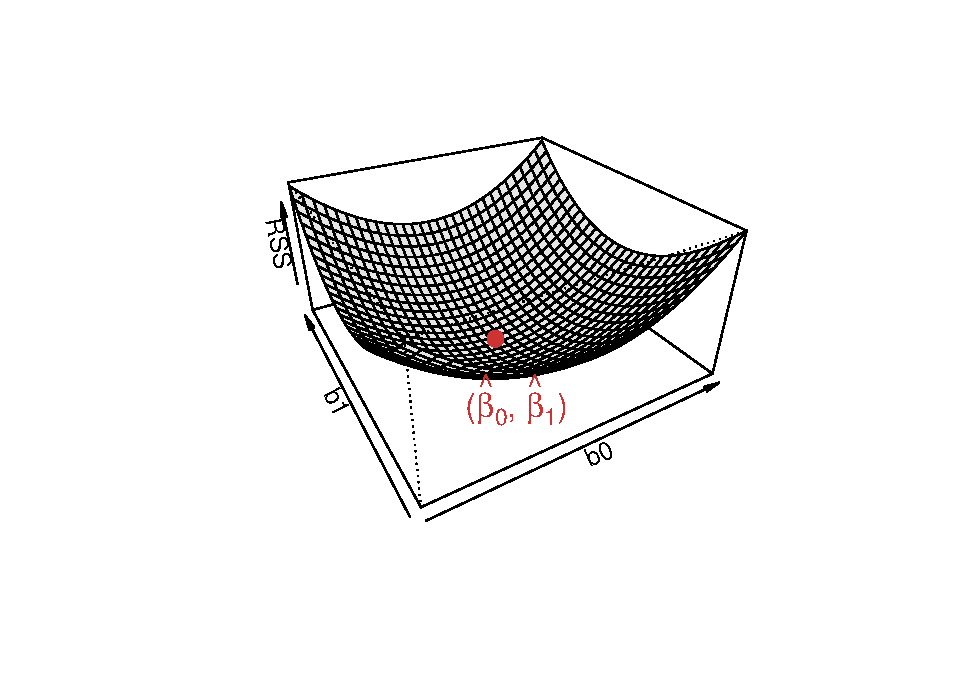
\includegraphics[width=0.8\linewidth]{Lab_6_files/figure-latex/unnamed-chunk-5-1} \end{center}

Odată ce avem estimatorii \((\hat\beta_0,\hat\beta_1)\) , putem defini:

\begin{itemize}
\tightlist
\item
  \emph{valorile prognozate} (\emph{fitted values})
  \(\hat Y_1,\ldots,\hat Y_n\) (valorile verticale pe dreapta de
  regresie), unde
\end{itemize}

\[
\hat Y_i=\hat\beta_0+\hat\beta_1X_i,\quad i=1,\ldots,n
\]

\begin{itemize}
\tightlist
\item
  \emph{reziduurile estimate} (\emph{estimated residuals})
  \(\hat \varepsilon_1,\ldots,\hat \varepsilon_n\) (distanțele verticale
  dintre punctele actuale \((X_i,Y_i)\) și cele prognozate
  \((X_i,\hat Y_i)\)), unde
\end{itemize}

\[
\hat\varepsilon_i=Y_i-\hat Y_i,\quad i=1,\ldots,n
\]

Estimatorul pentru \(\sigma^2\) este

\[
\hat{\sigma}^2 = \frac{RSS(\hat{\beta}_0,\hat{\beta}_1)}{n-2} = \frac{\sum_{i=1}^{n}\hat{\varepsilon}_i^2}{n-2}.
\] \#\# Funcția \texttt{lm()} din R

Pentru a rula modelul de regresie liniară simplă în R se folosește
funcția \texttt{lm()} (\emph{linear model}). Funcția \texttt{lm()} are
două argumente esențiale: \texttt{formula} și \texttt{data}.

\begin{longtable}[]{@{}ll@{}}
\toprule
\begin{minipage}[b]{0.18\columnwidth}\raggedright\strut
Argument\strut
\end{minipage} & \begin{minipage}[b]{0.67\columnwidth}\raggedright\strut
Descriere\strut
\end{minipage}\tabularnewline
\midrule
\endhead
\begin{minipage}[t]{0.18\columnwidth}\raggedright\strut
\texttt{formula}\strut
\end{minipage} & \begin{minipage}[t]{0.67\columnwidth}\raggedright\strut
O formulă de forma \(y \sim x_1 + x_2 + \ldots\), unde \(y\) este
variabila răspuns (dependentă) iar \(x_1,x_2,\ldots\) sunt variabilele
explicative (independente). Dacă vrem să includem toate coloanele (cu
excepția lui \(y\)) ca variabile explicative putem folosi
\(y \sim .\)\strut
\end{minipage}\tabularnewline
\begin{minipage}[t]{0.18\columnwidth}\raggedright\strut
\texttt{data}\strut
\end{minipage} & \begin{minipage}[t]{0.67\columnwidth}\raggedright\strut
Este setul de date în format \texttt{data.frame} care conține coloanele
specificate de formulă.\strut
\end{minipage}\tabularnewline
\bottomrule
\end{longtable}

Următorul tabel conține corespondențe între codul \texttt{R} și
conceptele statistice asociate modelului de regresie:

\begin{longtable}[]{@{}ll@{}}
\toprule
\begin{minipage}[b]{0.49\columnwidth}\raggedright\strut
\texttt{R}\strut
\end{minipage} & \begin{minipage}[b]{0.45\columnwidth}\raggedright\strut
Concepte statistice\strut
\end{minipage}\tabularnewline
\midrule
\endhead
\begin{minipage}[t]{0.49\columnwidth}\raggedright\strut
\texttt{x}\strut
\end{minipage} & \begin{minipage}[t]{0.45\columnwidth}\raggedright\strut
Variabilele predictor \(X_1,\ldots,X_n\)\strut
\end{minipage}\tabularnewline
\begin{minipage}[t]{0.49\columnwidth}\raggedright\strut
\texttt{y}\strut
\end{minipage} & \begin{minipage}[t]{0.45\columnwidth}\raggedright\strut
Răspunsul \(Y_1,\ldots,Y_n\)\strut
\end{minipage}\tabularnewline
\begin{minipage}[t]{0.49\columnwidth}\raggedright\strut
\texttt{data\ \textless{}-\ data.frame(x\ =\ x,\ y\ =\ y)}\strut
\end{minipage} & \begin{minipage}[t]{0.45\columnwidth}\raggedright\strut
Eșantionul \((X_1,Y_1),\ldots,(X_n,Y_n)\)\strut
\end{minipage}\tabularnewline
\begin{minipage}[t]{0.49\columnwidth}\raggedright\strut
\texttt{model\ \textless{}-\ lm(y\ \textasciitilde{}\ x,\ data\ =\ data)}\strut
\end{minipage} & \begin{minipage}[t]{0.45\columnwidth}\raggedright\strut
Modelul de regresie liniară simplă\strut
\end{minipage}\tabularnewline
\begin{minipage}[t]{0.49\columnwidth}\raggedright\strut
\texttt{model\$coefficients}\strut
\end{minipage} & \begin{minipage}[t]{0.45\columnwidth}\raggedright\strut
Coeficienții \(\hat\beta_0,\hat\beta_1\)\strut
\end{minipage}\tabularnewline
\begin{minipage}[t]{0.49\columnwidth}\raggedright\strut
\texttt{model\$residuals}\strut
\end{minipage} & \begin{minipage}[t]{0.45\columnwidth}\raggedright\strut
Valorile reziduale \(\hat\varepsilon_1,\ldots,\hat\varepsilon_n\)\strut
\end{minipage}\tabularnewline
\begin{minipage}[t]{0.49\columnwidth}\raggedright\strut
\texttt{model\$fitted.values}\strut
\end{minipage} & \begin{minipage}[t]{0.45\columnwidth}\raggedright\strut
Valorile fitate \(\hat Y_1,\ldots,\hat Y_n\)\strut
\end{minipage}\tabularnewline
\begin{minipage}[t]{0.49\columnwidth}\raggedright\strut
\texttt{model\$df.residual}\strut
\end{minipage} & \begin{minipage}[t]{0.45\columnwidth}\raggedright\strut
Gradele de libertate \(n-2\)\strut
\end{minipage}\tabularnewline
\begin{minipage}[t]{0.49\columnwidth}\raggedright\strut
\texttt{summaryModel\ \textless{}-\ summary(model)}\strut
\end{minipage} & \begin{minipage}[t]{0.45\columnwidth}\raggedright\strut
Sumarul modelului de regresie liniară\strut
\end{minipage}\tabularnewline
\begin{minipage}[t]{0.49\columnwidth}\raggedright\strut
\texttt{summaryModel\$sigma}\strut
\end{minipage} & \begin{minipage}[t]{0.45\columnwidth}\raggedright\strut
Estimatorul \(\hat\sigma\)\strut
\end{minipage}\tabularnewline
\begin{minipage}[t]{0.49\columnwidth}\raggedright\strut
\texttt{summaryModel\$r.squared}\strut
\end{minipage} & \begin{minipage}[t]{0.45\columnwidth}\raggedright\strut
Coeficientul de determinare \(R^2\)\strut
\end{minipage}\tabularnewline
\begin{minipage}[t]{0.49\columnwidth}\raggedright\strut
\texttt{summaryModel\$fstatistic}\strut
\end{minipage} & \begin{minipage}[t]{0.45\columnwidth}\raggedright\strut
Testul lui Fisher \(F\)\strut
\end{minipage}\tabularnewline
\begin{minipage}[t]{0.49\columnwidth}\raggedright\strut
\texttt{anova(model)}\strut
\end{minipage} & \begin{minipage}[t]{0.45\columnwidth}\raggedright\strut
Tabelul ANOVA\strut
\end{minipage}\tabularnewline
\bottomrule
\end{longtable}

\subsection{Aplicație}\label{aplicatie}

\begin{rmdexercise}
Ne propunem să investigăm relația dintre consumul de clorură de sodiu
(sarea de bucătărie) și tensiunea arterială la persoanele trecute de 65
de ani. Pentru aceasta vom folosi setul de date
\href{dataIn/saltBP.txt}{saltBP} care conține informații despre
tensiunea arterială a 25 de pacienți.
\end{rmdexercise}

Începem prin a înregistra setul de date

\begin{Shaded}
\begin{Highlighting}[]
\NormalTok{saltBP =}\StringTok{ }\KeywordTok{read.table}\NormalTok{(}\StringTok{"dataIn/saltBP.txt"}\NormalTok{, }\DataTypeTok{header =}\NormalTok{ T)}

\KeywordTok{summary}\NormalTok{(saltBP)}
\NormalTok{       BP             salt          saltLevel  }
\NormalTok{ Min.   }\OperatorTok{:}\FloatTok{128.3}\NormalTok{   Min.   }\OperatorTok{:}\StringTok{ }\FloatTok{1.130}\NormalTok{   Min.   }\OperatorTok{:}\FloatTok{0.0}  
\NormalTok{ 1st Qu.}\OperatorTok{:}\FloatTok{131.8}\NormalTok{   1st Qu.}\OperatorTok{:}\StringTok{ }\FloatTok{2.650}\NormalTok{   1st Qu.}\OperatorTok{:}\FloatTok{0.0}  
\NormalTok{ Median }\OperatorTok{:}\FloatTok{135.7}\NormalTok{   Median }\OperatorTok{:}\StringTok{ }\FloatTok{5.210}\NormalTok{   Median }\OperatorTok{:}\FloatTok{0.0}  
\NormalTok{ Mean   }\OperatorTok{:}\FloatTok{135.7}\NormalTok{   Mean   }\OperatorTok{:}\StringTok{ }\FloatTok{5.898}\NormalTok{   Mean   }\OperatorTok{:}\FloatTok{0.4}  
\NormalTok{ 3rd Qu.}\OperatorTok{:}\FloatTok{137.5}\NormalTok{   3rd Qu.}\OperatorTok{:}\StringTok{ }\FloatTok{8.680}\NormalTok{   3rd Qu.}\OperatorTok{:}\FloatTok{1.0}  
\NormalTok{ Max.   }\OperatorTok{:}\FloatTok{145.0}\NormalTok{   Max.   }\OperatorTok{:}\FloatTok{12.570}\NormalTok{   Max.   }\OperatorTok{:}\FloatTok{1.0}  
\end{Highlighting}
\end{Shaded}

și a ilustra grafic diagrama de împrăștiere

\begin{Shaded}
\begin{Highlighting}[]
\KeywordTok{plot}\NormalTok{(saltBP}\OperatorTok{$}\NormalTok{salt, saltBP}\OperatorTok{$}\NormalTok{BP, }
     \DataTypeTok{xlab =} \StringTok{"sare"}\NormalTok{, }
     \DataTypeTok{ylab =} \StringTok{"tensiunea arteriala"}\NormalTok{, }
     \DataTypeTok{col =} \StringTok{"brown3"}\NormalTok{, }
     \DataTypeTok{pch =} \DecValTok{16}\NormalTok{, }
     \DataTypeTok{bty=}\StringTok{"n"}\NormalTok{)}
\end{Highlighting}
\end{Shaded}

\begin{center}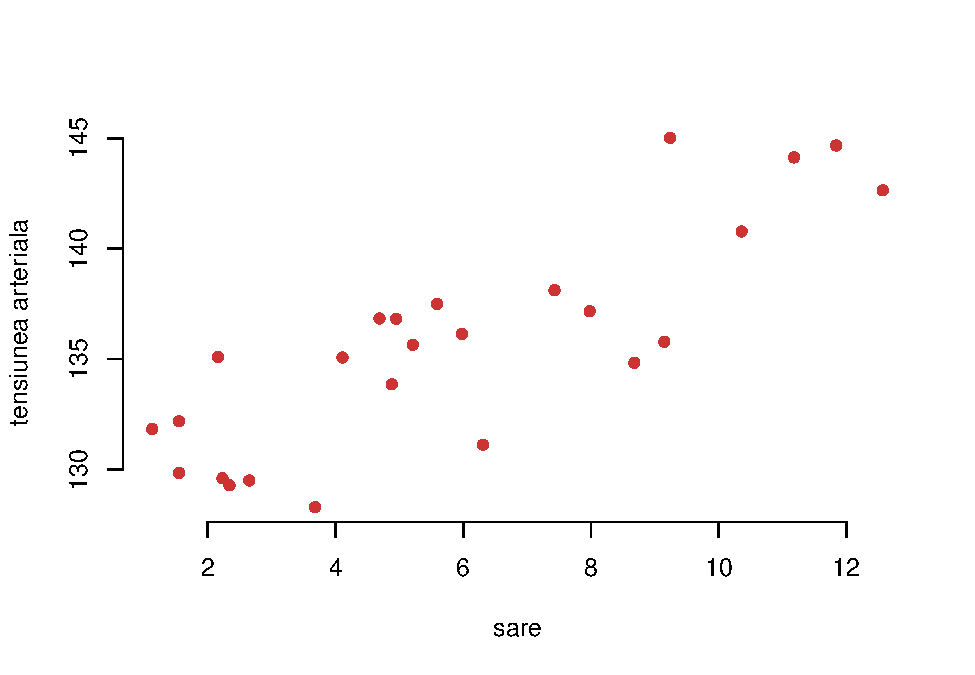
\includegraphics[width=0.8\linewidth]{Lab_6_files/figure-latex/unnamed-chunk-8-1} \end{center}

\subsubsection{Estimarea parametrilor}\label{estimarea-parametrilor}

Considerăm modelul de regresie \(Y = \beta_0 + \beta_1 X + \varepsilon\)
(unde \(X=\)\texttt{saltBP\$salt} iar \(Y=\)\texttt{saltBP\$BP}),
\(\varepsilon\sim \mathcal{N}(0,\sigma^2)\), a cărui parametrii sunt
\(\beta_0\), \(\beta_1\) și \(\sigma^2\).

Observăm că estimatorii parametrilor \(\beta_0\) și \(\beta_1\) sunt

\begin{Shaded}
\begin{Highlighting}[]
\CommentTok{# pentru b1}

\NormalTok{b1 =}\StringTok{ }\KeywordTok{cov}\NormalTok{(saltBP}\OperatorTok{$}\NormalTok{salt, saltBP}\OperatorTok{$}\NormalTok{BP)}\OperatorTok{/}\KeywordTok{var}\NormalTok{(saltBP}\OperatorTok{$}\NormalTok{salt)}
\KeywordTok{cat}\NormalTok{(}\StringTok{"b1 = "}\NormalTok{, b1, }\StringTok{"}\CharTok{\textbackslash{}n}\StringTok{"}\NormalTok{)}
\NormalTok{b1 =}\StringTok{  }\FloatTok{1.196894} 

\CommentTok{# sau }

\KeywordTok{sum}\NormalTok{((saltBP}\OperatorTok{$}\NormalTok{salt}\OperatorTok{-}\KeywordTok{mean}\NormalTok{(saltBP}\OperatorTok{$}\NormalTok{salt))}\OperatorTok{*}\NormalTok{(saltBP}\OperatorTok{$}\NormalTok{BP))}\OperatorTok{/}\KeywordTok{sum}\NormalTok{((saltBP}\OperatorTok{$}\NormalTok{salt}\OperatorTok{-}\KeywordTok{mean}\NormalTok{(saltBP}\OperatorTok{$}\NormalTok{salt))}\OperatorTok{^}\DecValTok{2}\NormalTok{)}
\NormalTok{[}\DecValTok{1}\NormalTok{] }\FloatTok{1.196894}

\CommentTok{# pentru b0}

\NormalTok{b0 =}\StringTok{ }\KeywordTok{mean}\NormalTok{(saltBP}\OperatorTok{$}\NormalTok{BP) }\OperatorTok{-}\StringTok{ }\NormalTok{b1}\OperatorTok{*}\KeywordTok{mean}\NormalTok{(saltBP}\OperatorTok{$}\NormalTok{salt)}
\KeywordTok{cat}\NormalTok{(}\StringTok{"b0 = "}\NormalTok{, b0)}
\NormalTok{b0 =}\StringTok{  }\FloatTok{128.6164}
\end{Highlighting}
\end{Shaded}

sau folosind funcția \texttt{lm()}:

\begin{Shaded}
\begin{Highlighting}[]
\NormalTok{saltBP_model =}\StringTok{ }\KeywordTok{lm}\NormalTok{(BP}\OperatorTok{~}\NormalTok{salt, }\DataTypeTok{data =}\NormalTok{ saltBP)}
\KeywordTok{names}\NormalTok{(saltBP_model)}
\NormalTok{ [}\DecValTok{1}\NormalTok{] }\StringTok{"coefficients"}  \StringTok{"residuals"}     \StringTok{"effects"}       \StringTok{"rank"}         
\NormalTok{ [}\DecValTok{5}\NormalTok{] }\StringTok{"fitted.values"} \StringTok{"assign"}        \StringTok{"qr"}            \StringTok{"df.residual"}  
\NormalTok{ [}\DecValTok{9}\NormalTok{] }\StringTok{"xlevels"}       \StringTok{"call"}          \StringTok{"terms"}         \StringTok{"model"}        
\end{Highlighting}
\end{Shaded}

\begin{Shaded}
\begin{Highlighting}[]
\NormalTok{saltBP_model}\OperatorTok{$}\NormalTok{coefficients}
\NormalTok{(Intercept)        salt }
 \FloatTok{128.616397}    \FloatTok{1.196894} 
\end{Highlighting}
\end{Shaded}

Dreapta de regresie este:

\begin{Shaded}
\begin{Highlighting}[]
\KeywordTok{plot}\NormalTok{(saltBP}\OperatorTok{$}\NormalTok{salt, saltBP}\OperatorTok{$}\NormalTok{BP, }
     \DataTypeTok{xlab =} \StringTok{"nivelul de sare"}\NormalTok{, }
     \DataTypeTok{ylab =} \StringTok{"tensiunea arteriala"}\NormalTok{, }
     \DataTypeTok{col =} \StringTok{"brown3"}\NormalTok{, }
     \DataTypeTok{pch =} \DecValTok{16}\NormalTok{, }
     \DataTypeTok{bty=}\StringTok{"n"}\NormalTok{, }
     \DataTypeTok{main =} \KeywordTok{paste}\NormalTok{(}\StringTok{"y = "}\NormalTok{, }\KeywordTok{format}\NormalTok{(b0, }\DataTypeTok{digits =} \DecValTok{4}\NormalTok{), }\StringTok{" + "}\NormalTok{, }\KeywordTok{format}\NormalTok{(b1, }\DataTypeTok{digits =} \DecValTok{4}\NormalTok{), }\StringTok{" x"}\NormalTok{))}

\KeywordTok{abline}\NormalTok{(}\DataTypeTok{a =}\NormalTok{ b0, }\DataTypeTok{b =}\NormalTok{ b1, }\DataTypeTok{col =} \StringTok{"grey"}\NormalTok{, }\DataTypeTok{lwd =} \DecValTok{2}\NormalTok{)}
\KeywordTok{points}\NormalTok{(}\KeywordTok{mean}\NormalTok{(saltBP}\OperatorTok{$}\NormalTok{salt), }\KeywordTok{mean}\NormalTok{(saltBP}\OperatorTok{$}\NormalTok{BP), }\DataTypeTok{pch =} \DecValTok{16}\NormalTok{, }\DataTypeTok{col =} \StringTok{"dark green"}\NormalTok{, }\DataTypeTok{cex =} \FloatTok{1.2}\NormalTok{)}
\KeywordTok{text}\NormalTok{(}\KeywordTok{mean}\NormalTok{(saltBP}\OperatorTok{$}\NormalTok{salt), }\KeywordTok{mean}\NormalTok{(saltBP}\OperatorTok{$}\NormalTok{BP)}\OperatorTok{-}\FloatTok{1.3}\NormalTok{, }\DataTypeTok{col =} \StringTok{"dark green"}\NormalTok{, }\DataTypeTok{cex =} \FloatTok{1.2}\NormalTok{, }
     \DataTypeTok{labels =} \KeywordTok{expression}\NormalTok{(}\KeywordTok{paste}\NormalTok{(}\StringTok{"("}\NormalTok{, }\KeywordTok{bar}\NormalTok{(x), }\StringTok{","}\NormalTok{, }\KeywordTok{bar}\NormalTok{(y),}\StringTok{")"}\NormalTok{)))}
\end{Highlighting}
\end{Shaded}

\begin{center}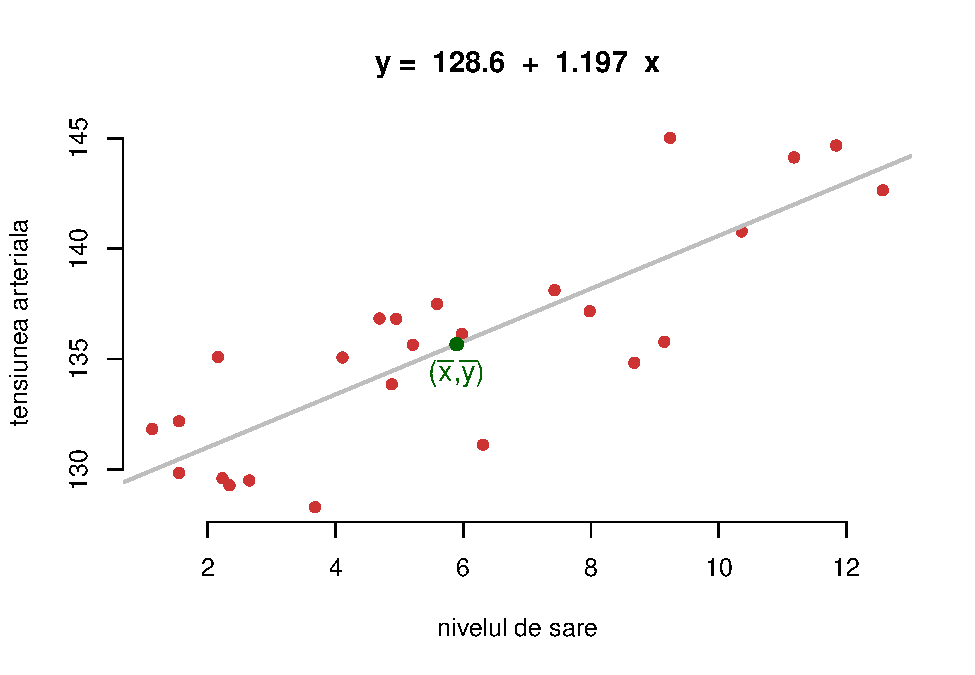
\includegraphics[width=0.8\linewidth]{Lab_6_files/figure-latex/unnamed-chunk-12-1} \end{center}

De asemenea pentru calculul estimatorului lui \(\sigma\)
(\(\hat{\sigma}\)) avem

\begin{Shaded}
\begin{Highlighting}[]
\NormalTok{n =}\StringTok{ }\KeywordTok{length}\NormalTok{(saltBP}\OperatorTok{$}\NormalTok{BP)}
\NormalTok{e_hat =}\StringTok{ }\NormalTok{saltBP}\OperatorTok{$}\NormalTok{BP }\OperatorTok{-}\StringTok{ }\NormalTok{(b0}\OperatorTok{+}\NormalTok{b1}\OperatorTok{*}\NormalTok{saltBP}\OperatorTok{$}\NormalTok{salt)}

\NormalTok{rss =}\StringTok{ }\KeywordTok{sum}\NormalTok{(e_hat}\OperatorTok{^}\DecValTok{2}\NormalTok{)}

\NormalTok{sigma_hat =}\StringTok{ }\KeywordTok{sqrt}\NormalTok{(rss}\OperatorTok{/}\NormalTok{(n}\OperatorTok{-}\DecValTok{2}\NormalTok{))}
\NormalTok{sigma_hat}
\NormalTok{[}\DecValTok{1}\NormalTok{] }\FloatTok{2.745374}
\end{Highlighting}
\end{Shaded}

sau cu ajutorul funcției \texttt{lm()}

\begin{Shaded}
\begin{Highlighting}[]
\KeywordTok{sqrt}\NormalTok{(}\KeywordTok{deviance}\NormalTok{(saltBP_model)}\OperatorTok{/}\KeywordTok{df.residual}\NormalTok{(saltBP_model))}
\NormalTok{[}\DecValTok{1}\NormalTok{] }\FloatTok{2.745374}
\end{Highlighting}
\end{Shaded}

sau încă

\begin{Shaded}
\begin{Highlighting}[]
\NormalTok{saltBP_model_summary =}\StringTok{ }\KeywordTok{summary}\NormalTok{(saltBP_model)}

\NormalTok{saltBP_model_summary}\OperatorTok{$}\NormalTok{sigma}
\NormalTok{[}\DecValTok{1}\NormalTok{] }\FloatTok{2.745374}
\end{Highlighting}
\end{Shaded}

\subsubsection{Intervale de încredere pentru
parametrii}\label{intervale-de-incredere-pentru-parametrii}

Repartițiile lui \(\hat\beta_0\) și \(\hat\beta_1\) sunt

\[
\hat\beta_0\sim\mathcal{N}\left(\beta_0,\mathrm{SE}(\hat\beta_0)^2\right),\quad\hat\beta_1\sim\mathcal{N}\left(\beta_1,\mathrm{SE}(\hat\beta_1)^2\right)
\]

unde

\[
\mathrm{SE}(\hat\beta_0)^2=\frac{\sigma^2}{n}\left[1+\frac{\bar X^2}{s_{xx}^2}\right],\quad \mathrm{SE}(\hat\beta_1)^2=\frac{\sigma^2}{ns_{xx}^2}.
\]

Folosind estimatorul \(\hat\sigma^2\) pentru \(\sigma^2\) obținem că

\[
\frac{\hat\beta_0-\beta_0}{\hat{\mathrm{SE}}(\hat\beta_0)}\sim t_{n-2},\quad\frac{\hat\beta_1-\beta_1}{\hat{\mathrm{SE}}(\hat\beta_1)}\sim t_{n-2}
\]

unde

\[
\hat{\mathrm{SE}}(\hat\beta_0)^2=\frac{\hat\sigma^2}{n}\left[1+\frac{\bar X^2}{s_{xx}^2}\right],\quad \hat{\mathrm{SE}}(\hat\beta_1)^2=\frac{\hat\sigma^2}{ns_{xx}^2}
\]

prin urmare, intervalele de încredere de nivel \(1-\alpha\) pentru
\(\beta_0\) și \(\beta_1\) sunt

\[
IC = \left(\hat\beta_j\pm\hat{\mathrm{SE}}(\hat\beta_j)t_{n-2;1-\alpha/2}\right),\quad j=0,1.
\]

În R avem

\begin{Shaded}
\begin{Highlighting}[]
\NormalTok{alpha =}\StringTok{ }\FloatTok{0.05}

\CommentTok{# trebuie avut grija ca functia var si sd se calculeaza }
\CommentTok{# impartind la (n-1) si nu la n !!!}

\NormalTok{se_b0 =}\StringTok{ }\KeywordTok{sqrt}\NormalTok{(sigma_hat}\OperatorTok{^}\DecValTok{2}\OperatorTok{*}\NormalTok{(}\DecValTok{1}\OperatorTok{/}\NormalTok{n}\OperatorTok{+}\KeywordTok{mean}\NormalTok{(saltBP}\OperatorTok{$}\NormalTok{salt)}\OperatorTok{^}\DecValTok{2}\OperatorTok{/}\NormalTok{((n}\OperatorTok{-}\DecValTok{1}\NormalTok{)}\OperatorTok{*}\KeywordTok{var}\NormalTok{(saltBP}\OperatorTok{$}\NormalTok{salt))))}
\NormalTok{se_b1 =}\StringTok{ }\KeywordTok{sqrt}\NormalTok{(sigma_hat}\OperatorTok{^}\DecValTok{2}\OperatorTok{/}\NormalTok{((n}\OperatorTok{-}\DecValTok{1}\NormalTok{)}\OperatorTok{*}\KeywordTok{var}\NormalTok{(saltBP}\OperatorTok{$}\NormalTok{salt)))}

\NormalTok{lw_b0 =}\StringTok{ }\NormalTok{b0 }\OperatorTok{-}\StringTok{ }\KeywordTok{qt}\NormalTok{(}\DecValTok{1}\OperatorTok{-}\NormalTok{alpha}\OperatorTok{/}\DecValTok{2}\NormalTok{, n}\OperatorTok{-}\DecValTok{2}\NormalTok{)}\OperatorTok{*}\NormalTok{se_b0}
\NormalTok{up_b0 =}\StringTok{ }\NormalTok{b0 }\OperatorTok{+}\StringTok{ }\KeywordTok{qt}\NormalTok{(}\DecValTok{1}\OperatorTok{-}\NormalTok{alpha}\OperatorTok{/}\DecValTok{2}\NormalTok{, n}\OperatorTok{-}\DecValTok{2}\NormalTok{)}\OperatorTok{*}\NormalTok{se_b0}

\KeywordTok{cat}\NormalTok{(}\StringTok{"CI pentru b0 este ("}\NormalTok{, lw_b0, }\StringTok{", "}\NormalTok{, up_b0, }\StringTok{")}\CharTok{\textbackslash{}n}\StringTok{"}\NormalTok{)}
\NormalTok{CI pentru b0 }\KeywordTok{este}\NormalTok{ ( }\FloatTok{126.337}\NormalTok{ ,  }\FloatTok{130.8958}\NormalTok{ )}

\NormalTok{lw_b1 =}\StringTok{ }\NormalTok{b1 }\OperatorTok{-}\StringTok{ }\KeywordTok{qt}\NormalTok{(}\DecValTok{1}\OperatorTok{-}\NormalTok{alpha}\OperatorTok{/}\DecValTok{2}\NormalTok{, n}\OperatorTok{-}\DecValTok{2}\NormalTok{)}\OperatorTok{*}\NormalTok{se_b1}
\NormalTok{up_b1 =}\StringTok{ }\NormalTok{b1 }\OperatorTok{+}\StringTok{ }\KeywordTok{qt}\NormalTok{(}\DecValTok{1}\OperatorTok{-}\NormalTok{alpha}\OperatorTok{/}\DecValTok{2}\NormalTok{, n}\OperatorTok{-}\DecValTok{2}\NormalTok{)}\OperatorTok{*}\NormalTok{se_b1}
  
\KeywordTok{cat}\NormalTok{(}\StringTok{"CI pentru b1 este ("}\NormalTok{, lw_b1, }\StringTok{", "}\NormalTok{, up_b1, }\StringTok{")"}\NormalTok{)}
\NormalTok{CI pentru b1 }\KeywordTok{este}\NormalTok{ ( }\FloatTok{0.8617951}\NormalTok{ ,  }\FloatTok{1.531993}\NormalTok{ )}
\end{Highlighting}
\end{Shaded}

Același rezultat se obține apelând funcția \texttt{confint()} :

\begin{Shaded}
\begin{Highlighting}[]
\KeywordTok{confint}\NormalTok{(saltBP_model)}
                  \FloatTok{2.5} \OperatorTok
\NormalTok{(Intercept) }\FloatTok{126.3369606} \FloatTok{130.895834}
\NormalTok{salt          }\FloatTok{0.8617951}   \FloatTok{1.531993}
\end{Highlighting}
\end{Shaded}

Putem construi și o regiune de încredere pentru perechea
\((\beta_0, \beta_1)\):

\begin{Shaded}
\begin{Highlighting}[]
\CommentTok{# library(ellipse)}

\KeywordTok{par}\NormalTok{(}\DataTypeTok{bty =} \StringTok{"n"}\NormalTok{)}
\KeywordTok{confidenceEllipse}\NormalTok{(saltBP_model,}
                  \DataTypeTok{xlab =} \KeywordTok{expression}\NormalTok{(beta[}\DecValTok{0}\NormalTok{]), }
                  \DataTypeTok{ylab =} \KeywordTok{expression}\NormalTok{(beta[}\DecValTok{1}\NormalTok{]),}
                  \DataTypeTok{col =} \StringTok{"grey30"}\NormalTok{) }
\KeywordTok{points}\NormalTok{(}\KeywordTok{coef}\NormalTok{(saltBP_model)[}\DecValTok{1}\NormalTok{], }\KeywordTok{coef}\NormalTok{(saltBP_model)[}\DecValTok{2}\NormalTok{], }
       \DataTypeTok{pch =} \DecValTok{18}\NormalTok{, }\DataTypeTok{col =} \StringTok{"brown3"}\NormalTok{,}
       \DataTypeTok{cex =} \DecValTok{2}\NormalTok{)}
\KeywordTok{abline}\NormalTok{(}\DataTypeTok{v =} \KeywordTok{confint}\NormalTok{(saltBP_model)[}\DecValTok{1}\NormalTok{,], }\DataTypeTok{lty =} \DecValTok{2}\NormalTok{)}
\KeywordTok{abline}\NormalTok{(}\DataTypeTok{h =} \KeywordTok{confint}\NormalTok{(saltBP_model)[}\DecValTok{2}\NormalTok{,], }\DataTypeTok{lty =} \DecValTok{2}\NormalTok{)}
\end{Highlighting}
\end{Shaded}

\begin{center}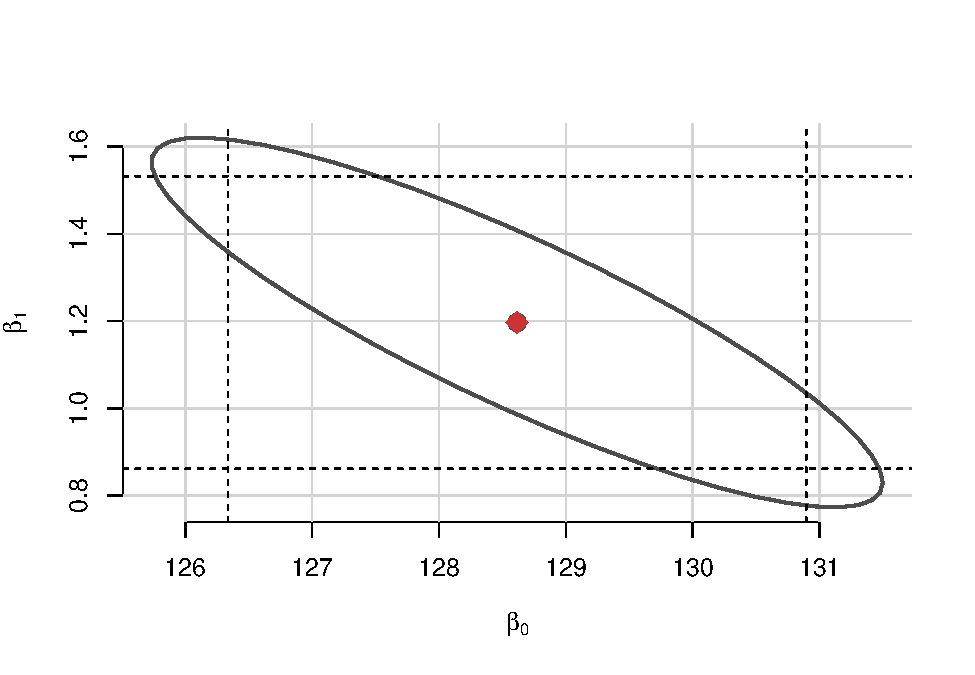
\includegraphics[width=0.8\linewidth]{Lab_6_files/figure-latex/unnamed-chunk-18-1} \end{center}

\subsubsection{ANOVA pentru regresie}\label{anova-pentru-regresie}

Este predictorul \(X\) folositor în prezicerea răspunsului \(Y\) ? Vrem
să testăm ipoteza nulă \(H_0:\;\beta_1=0\).

Introducem următoarele \emph{sume de abateri pătratice}:

\begin{itemize}
\tightlist
\item
  \(SS_T=\sum_{i=1}^n\left(Y_i-\bar Y\right)^2\), \textbf{suma
  abaterilor pătratice totală} (variația totală a lui
  \(Y_1,\ldots,Y_n\)).
\item
  \(SS_{reg}=\sum_{i=1}^n\left(\hat Y_i-\bar Y\right)^2\), \textbf{suma
  abaterilor pătratice de regresie} (variabilitatea explicată de dreapta
  de regresie)
\item
  \(RSS=\sum_{i=1}^n\left(Y_i-\hat Y_i\right)^2\), \textbf{suma
  abaterilor pătratice reziduale}
\end{itemize}

Avem următoarea descompunere ANOVA

\[
\underbrace{SS_T}_{\text{Variația lui }Y_i} = \underbrace{SS_{reg}}_{\text{Variația lui }\hat Y_i} + \underbrace{RSS}_{\text{Variația lui }\hat \varepsilon_i} 
\]

și tabelul ANOVA corespunzător

\begin{longtable}[]{@{}llllll@{}}
\toprule
& Df & SS & MS & \(F\) & \(p\)-value\tabularnewline
\midrule
\endhead
Predictor & \(1\) & \(SS_{reg}\) & \(\frac{SS_{reg}}{1}\) &
\(\frac{SS_{reg}/1}{RSS/(n-2)}\) & \(p\)\tabularnewline
Residuuri & \(n - 2\) & \(RSS\) & \(\frac{RSS}{n-2}\) & &\tabularnewline
\bottomrule
\end{longtable}

unde sub ipoteza nulă, \(H_0:\,\beta_1 = 0\), avem

\[
  F=\frac{SS_{reg}/1}{RSS/(n-2)}\stackrel{H_0}{\sim} F_{1,n-2}
\] Descompunerea ANOVA pentru problema noastră poate fi ilustrată
astfel:

\begin{enumerate}
\def\labelenumi{\alph{enumi})}
\tightlist
\item
  \emph{suma abaterilor pătratice totală}:
\end{enumerate}

\begin{Shaded}
\begin{Highlighting}[]
\KeywordTok{plot}\NormalTok{(saltBP}\OperatorTok{$}\NormalTok{salt, saltBP}\OperatorTok{$}\NormalTok{BP, }\DataTypeTok{pch =} \DecValTok{16}\NormalTok{, }\DataTypeTok{type =} \StringTok{"n"}\NormalTok{,}
     \DataTypeTok{main =} \KeywordTok{paste}\NormalTok{(}\StringTok{"SST ="}\NormalTok{, }\KeywordTok{round}\NormalTok{(}\KeywordTok{sum}\NormalTok{((saltBP}\OperatorTok{$}\NormalTok{BP }\OperatorTok{-}\StringTok{ }\KeywordTok{mean}\NormalTok{(saltBP}\OperatorTok{$}\NormalTok{BP))}\OperatorTok{^}\DecValTok{2}\NormalTok{), }\DecValTok{2}\NormalTok{)), }
     \DataTypeTok{col.main =} \StringTok{"brown4"}\NormalTok{, }
     \DataTypeTok{xlab =} \StringTok{"nivelul de sare"}\NormalTok{, }
     \DataTypeTok{ylab =} \StringTok{"tensiunea arteriala"}\NormalTok{, }
     \DataTypeTok{bty =} \StringTok{"n"}\NormalTok{)}

\KeywordTok{abline}\NormalTok{(saltBP_model}\OperatorTok{$}\NormalTok{coefficients, }\DataTypeTok{col =} \StringTok{"grey30"}\NormalTok{, }\DataTypeTok{lwd =} \DecValTok{2}\NormalTok{)}
\KeywordTok{abline}\NormalTok{(}\DataTypeTok{h =} \KeywordTok{mean}\NormalTok{(saltBP}\OperatorTok{$}\NormalTok{BP), }\DataTypeTok{col =} \StringTok{"brown2"}\NormalTok{, }\DataTypeTok{lty =} \DecValTok{2}\NormalTok{)}

\KeywordTok{segments}\NormalTok{(}\DataTypeTok{x0 =}\NormalTok{ saltBP}\OperatorTok{$}\NormalTok{salt, }\DataTypeTok{y0 =} \KeywordTok{mean}\NormalTok{(saltBP}\OperatorTok{$}\NormalTok{BP), }
         \DataTypeTok{x1 =}\NormalTok{ saltBP}\OperatorTok{$}\NormalTok{salt, }\DataTypeTok{y1 =}\NormalTok{ saltBP}\OperatorTok{$}\NormalTok{BP, }
         \DataTypeTok{col =} \StringTok{"grey50"}\NormalTok{, }\DataTypeTok{lwd =} \DecValTok{2}\NormalTok{, }\DataTypeTok{lty =} \DecValTok{2}\NormalTok{)}

\KeywordTok{legend}\NormalTok{(}\StringTok{"topleft"}\NormalTok{, }
       \DataTypeTok{legend =} \KeywordTok{expression}\NormalTok{(}\StringTok{"Dreapta de regresie"}\NormalTok{, }\StringTok{"Media esantionului "} \OperatorTok{*}\StringTok{ }\KeywordTok{bar}\NormalTok{(Y),}
\NormalTok{                                      (Y[i] }\OperatorTok{-}\StringTok{ }\KeywordTok{bar}\NormalTok{(Y))}\OperatorTok{^}\DecValTok{2}\NormalTok{), }
       \DataTypeTok{lwd =} \KeywordTok{c}\NormalTok{(}\DecValTok{2}\NormalTok{, }\DecValTok{1}\NormalTok{, }\DecValTok{2}\NormalTok{),}
       \DataTypeTok{col =} \KeywordTok{c}\NormalTok{(}\StringTok{"grey30"}\NormalTok{, }\StringTok{"brown2"}\NormalTok{, }\StringTok{"grey50"}\NormalTok{), }
       \DataTypeTok{lty =} \KeywordTok{c}\NormalTok{(}\DecValTok{1}\NormalTok{, }\DecValTok{2}\NormalTok{, }\DecValTok{2}\NormalTok{), }
       \DataTypeTok{bty =} \StringTok{"n"}\NormalTok{)}

\KeywordTok{points}\NormalTok{(saltBP}\OperatorTok{$}\NormalTok{salt, saltBP}\OperatorTok{$}\NormalTok{BP, }\DataTypeTok{pch =} \DecValTok{16}\NormalTok{, }\DataTypeTok{col =} \StringTok{"brown3"}\NormalTok{)}
\end{Highlighting}
\end{Shaded}

\begin{center}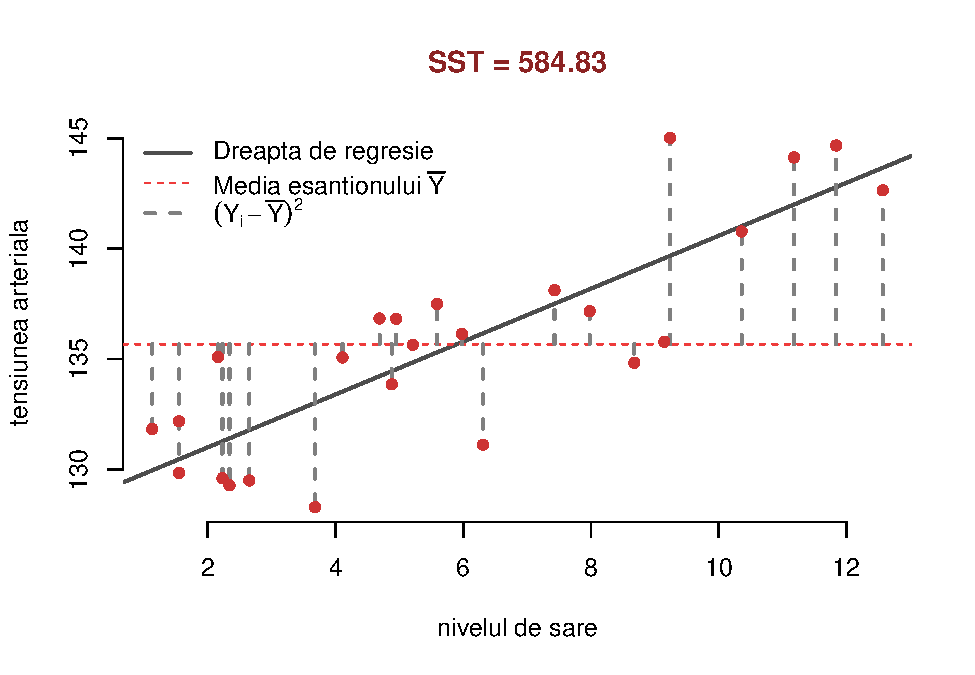
\includegraphics[width=0.8\linewidth]{Lab_6_files/figure-latex/unnamed-chunk-19-1} \end{center}

\begin{enumerate}
\def\labelenumi{\alph{enumi})}
\setcounter{enumi}{1}
\tightlist
\item
  \emph{suma abaterilor pătratice de regresie}
\end{enumerate}

\begin{Shaded}
\begin{Highlighting}[]
\KeywordTok{plot}\NormalTok{(saltBP}\OperatorTok{$}\NormalTok{salt, saltBP}\OperatorTok{$}\NormalTok{BP, }\DataTypeTok{pch =} \DecValTok{16}\NormalTok{, }\DataTypeTok{type =} \StringTok{"n"}\NormalTok{,}
     \DataTypeTok{main =} \KeywordTok{paste}\NormalTok{(}\StringTok{"SSreg ="}\NormalTok{, }
                  \KeywordTok{round}\NormalTok{(}\KeywordTok{sum}\NormalTok{((saltBP_model}\OperatorTok{$}\NormalTok{fitted.values }\OperatorTok{-}\StringTok{ }\KeywordTok{mean}\NormalTok{(saltBP}\OperatorTok{$}\NormalTok{BP))}\OperatorTok{^}\DecValTok{2}\NormalTok{), }\DecValTok{2}\NormalTok{)), }
     \DataTypeTok{col.main =} \StringTok{"forestgreen"}\NormalTok{, }
     \DataTypeTok{xlab =} \StringTok{"nivelul de sare"}\NormalTok{, }
     \DataTypeTok{ylab =} \StringTok{"tensiunea arteriala"}\NormalTok{, }
     \DataTypeTok{bty =} \StringTok{"n"}\NormalTok{)}

\KeywordTok{abline}\NormalTok{(saltBP_model}\OperatorTok{$}\NormalTok{coefficients, }\DataTypeTok{col =} \StringTok{"grey30"}\NormalTok{, }\DataTypeTok{lwd =} \DecValTok{2}\NormalTok{)}
\KeywordTok{abline}\NormalTok{(}\DataTypeTok{h =} \KeywordTok{mean}\NormalTok{(saltBP}\OperatorTok{$}\NormalTok{BP), }\DataTypeTok{col =} \StringTok{"brown2"}\NormalTok{, }\DataTypeTok{lty =} \DecValTok{2}\NormalTok{)}

\KeywordTok{segments}\NormalTok{(}\DataTypeTok{x0 =}\NormalTok{ saltBP}\OperatorTok{$}\NormalTok{salt, }\DataTypeTok{y0 =} \KeywordTok{mean}\NormalTok{(saltBP}\OperatorTok{$}\NormalTok{BP), }
         \DataTypeTok{x1 =}\NormalTok{ saltBP}\OperatorTok{$}\NormalTok{salt, }\DataTypeTok{y1 =}\NormalTok{ saltBP_model}\OperatorTok{$}\NormalTok{fitted.values, }
         \DataTypeTok{col =} \StringTok{"forestgreen"}\NormalTok{, }\DataTypeTok{lwd =} \DecValTok{2}\NormalTok{, }\DataTypeTok{lty =} \DecValTok{2}\NormalTok{)}

\KeywordTok{points}\NormalTok{(saltBP}\OperatorTok{$}\NormalTok{salt, saltBP_model}\OperatorTok{$}\NormalTok{fitted.values, }\DataTypeTok{pch =} \DecValTok{16}\NormalTok{, }\DataTypeTok{col =} \StringTok{"forestgreen"}\NormalTok{)}

\KeywordTok{legend}\NormalTok{(}\StringTok{"topleft"}\NormalTok{, }
       \DataTypeTok{legend =} \KeywordTok{expression}\NormalTok{(}\StringTok{"Dreapta de regresie"}\NormalTok{, }\StringTok{"Media esantionului "} \OperatorTok{*}\StringTok{ }\KeywordTok{bar}\NormalTok{(Y),}
\NormalTok{                                      (}\KeywordTok{hat}\NormalTok{(Y)[i] }\OperatorTok{-}\StringTok{ }\KeywordTok{bar}\NormalTok{(Y))}\OperatorTok{^}\DecValTok{2}\NormalTok{), }
       \DataTypeTok{lwd =} \KeywordTok{c}\NormalTok{(}\DecValTok{2}\NormalTok{, }\DecValTok{1}\NormalTok{, }\DecValTok{2}\NormalTok{),}
       \DataTypeTok{col =} \KeywordTok{c}\NormalTok{(}\StringTok{"grey30"}\NormalTok{, }\StringTok{"brown2"}\NormalTok{, }\StringTok{"forestgreen"}\NormalTok{), }
       \DataTypeTok{lty =} \KeywordTok{c}\NormalTok{(}\DecValTok{1}\NormalTok{, }\DecValTok{2}\NormalTok{, }\DecValTok{2}\NormalTok{), }
       \DataTypeTok{bty =} \StringTok{"n"}\NormalTok{)}

\KeywordTok{points}\NormalTok{(saltBP}\OperatorTok{$}\NormalTok{salt, saltBP}\OperatorTok{$}\NormalTok{BP, }\DataTypeTok{pch =} \DecValTok{16}\NormalTok{, }\DataTypeTok{col =} \StringTok{"brown3"}\NormalTok{)}
\end{Highlighting}
\end{Shaded}

\begin{center}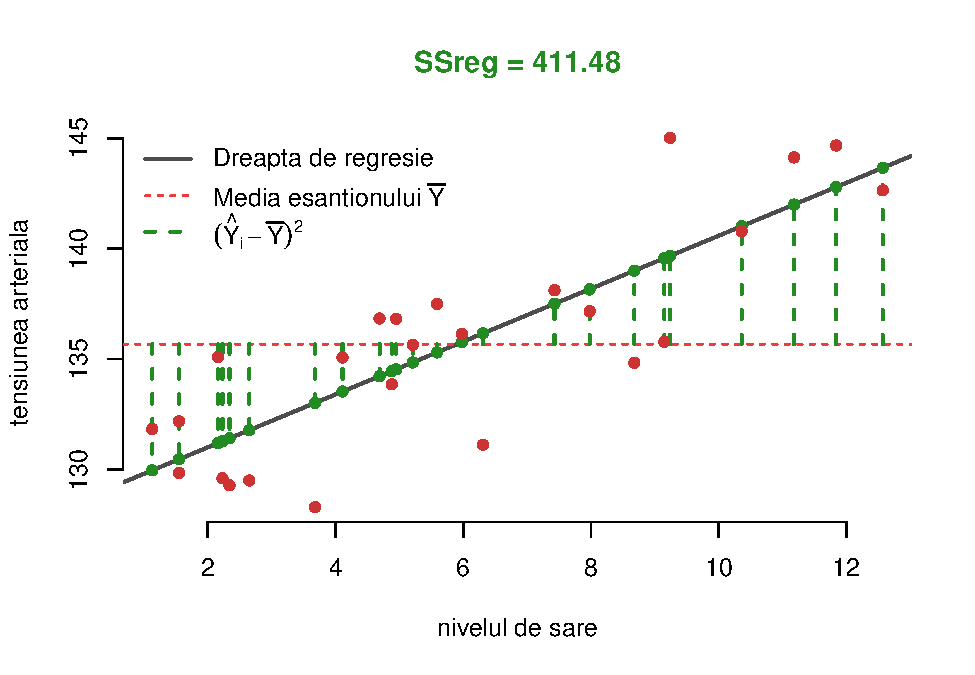
\includegraphics[width=0.8\linewidth]{Lab_6_files/figure-latex/unnamed-chunk-20-1} \end{center}

\begin{enumerate}
\def\labelenumi{\alph{enumi})}
\setcounter{enumi}{2}
\tightlist
\item
  \emph{suma abaterilor pătratice reziduale}
\end{enumerate}

\begin{Shaded}
\begin{Highlighting}[]
\KeywordTok{plot}\NormalTok{(saltBP}\OperatorTok{$}\NormalTok{salt, saltBP}\OperatorTok{$}\NormalTok{BP, }\DataTypeTok{pch =} \DecValTok{16}\NormalTok{, }\DataTypeTok{type =} \StringTok{"n"}\NormalTok{,}
     \DataTypeTok{main =} \KeywordTok{paste}\NormalTok{(}\StringTok{"RSS ="}\NormalTok{, }
                  \KeywordTok{round}\NormalTok{(}\KeywordTok{sum}\NormalTok{((saltBP}\OperatorTok{$}\NormalTok{BP }\OperatorTok{-}\StringTok{ }\NormalTok{saltBP_model}\OperatorTok{$}\NormalTok{fitted.values)}\OperatorTok{^}\DecValTok{2}\NormalTok{), }\DecValTok{2}\NormalTok{)), }
     \DataTypeTok{col.main =} \StringTok{"orange"}\NormalTok{, }
     \DataTypeTok{xlab =} \StringTok{"nivelul de sare"}\NormalTok{, }
     \DataTypeTok{ylab =} \StringTok{"tensiunea arteriala"}\NormalTok{, }
     \DataTypeTok{bty =} \StringTok{"n"}\NormalTok{)}

\KeywordTok{abline}\NormalTok{(saltBP_model}\OperatorTok{$}\NormalTok{coefficients, }\DataTypeTok{col =} \StringTok{"grey30"}\NormalTok{, }\DataTypeTok{lwd =} \DecValTok{2}\NormalTok{)}

\KeywordTok{segments}\NormalTok{(}\DataTypeTok{x0 =}\NormalTok{ saltBP}\OperatorTok{$}\NormalTok{salt, }\DataTypeTok{y0 =}\NormalTok{ saltBP}\OperatorTok{$}\NormalTok{BP, }
         \DataTypeTok{x1 =}\NormalTok{ saltBP}\OperatorTok{$}\NormalTok{salt, }\DataTypeTok{y1 =}\NormalTok{ saltBP_model}\OperatorTok{$}\NormalTok{fitted.values, }
         \DataTypeTok{col =} \StringTok{"orange"}\NormalTok{, }\DataTypeTok{lwd =} \DecValTok{2}\NormalTok{, }\DataTypeTok{lty =} \DecValTok{2}\NormalTok{)}

\KeywordTok{points}\NormalTok{(saltBP}\OperatorTok{$}\NormalTok{salt, saltBP_model}\OperatorTok{$}\NormalTok{fitted.values, }\DataTypeTok{pch =} \DecValTok{16}\NormalTok{, }\DataTypeTok{col =} \StringTok{"orange"}\NormalTok{)}

\KeywordTok{legend}\NormalTok{(}\StringTok{"topleft"}\NormalTok{, }
       \DataTypeTok{legend =} \KeywordTok{expression}\NormalTok{(}\StringTok{"Dreapta de regresie"}\NormalTok{, (}\KeywordTok{hat}\NormalTok{(Y)[i] }\OperatorTok{-}\StringTok{ }\NormalTok{Y[i])}\OperatorTok{^}\DecValTok{2}\NormalTok{), }
       \DataTypeTok{lwd =} \KeywordTok{c}\NormalTok{(}\DecValTok{2}\NormalTok{, }\DecValTok{2}\NormalTok{),}
       \DataTypeTok{col =} \KeywordTok{c}\NormalTok{(}\StringTok{"grey30"}\NormalTok{, }\StringTok{"orange"}\NormalTok{), }
       \DataTypeTok{lty =} \KeywordTok{c}\NormalTok{(}\DecValTok{1}\NormalTok{, }\DecValTok{2}\NormalTok{), }
       \DataTypeTok{bty =} \StringTok{"n"}\NormalTok{)}

\KeywordTok{points}\NormalTok{(saltBP}\OperatorTok{$}\NormalTok{salt, saltBP}\OperatorTok{$}\NormalTok{BP, }\DataTypeTok{pch =} \DecValTok{16}\NormalTok{, }\DataTypeTok{col =} \StringTok{"brown3"}\NormalTok{)}
\end{Highlighting}
\end{Shaded}

\begin{center}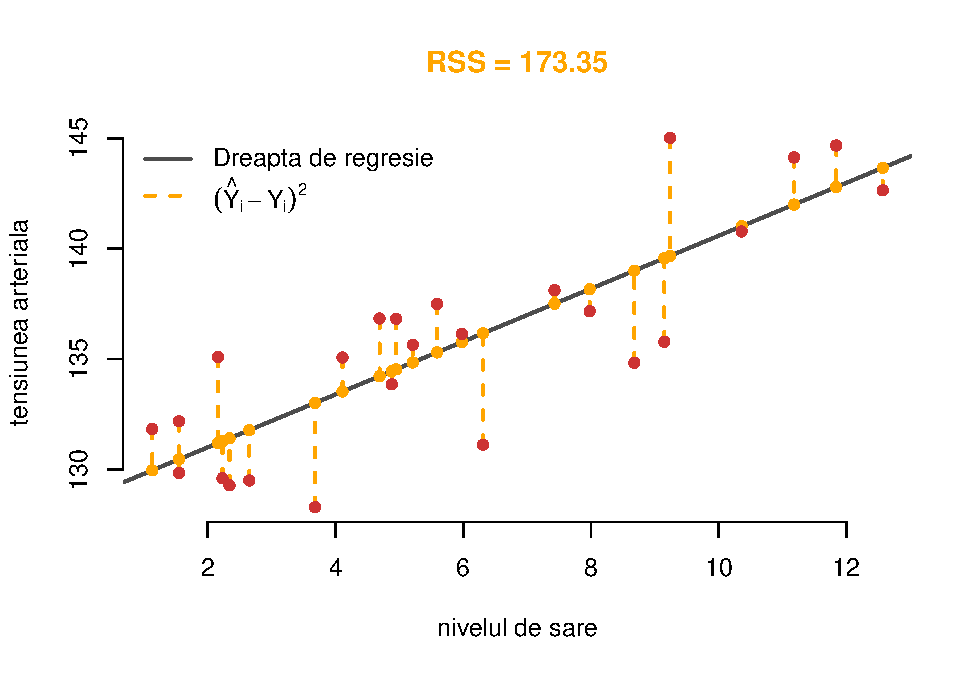
\includegraphics[width=0.8\linewidth]{Lab_6_files/figure-latex/unnamed-chunk-21-1} \end{center}

Tabelul ANOVA se obține prin

\begin{Shaded}
\begin{Highlighting}[]
\CommentTok{# tabel ANOVA }
\KeywordTok{anova}\NormalTok{(saltBP_model)}
\NormalTok{Analysis of Variance Table}

\NormalTok{Response}\OperatorTok{:}\StringTok{ }\NormalTok{BP}
\NormalTok{          Df Sum Sq Mean Sq F value    }\KeywordTok{Pr}\NormalTok{(}\OperatorTok{>}\NormalTok{F)    }
\NormalTok{salt       }\DecValTok{1} \FloatTok{411.48}  \FloatTok{411.48}  \FloatTok{54.594} \FloatTok{1.631e-07} \OperatorTok{**}\ErrorTok{*}
\NormalTok{Residuals }\DecValTok{23} \FloatTok{173.35}    \FloatTok{7.54}                      
\OperatorTok{---}
\NormalTok{Signif. codes}\OperatorTok{:}\StringTok{  }\DecValTok{0} \StringTok{'***'} \FloatTok{0.001} \StringTok{'**'} \FloatTok{0.01} \StringTok{'*'} \FloatTok{0.05} \StringTok{'.'} \FloatTok{0.1} \StringTok{' '} \DecValTok{1}
\end{Highlighting}
\end{Shaded}

Definiția \emph{coeficientului de determinare} \(R^2\) este strâns
legată de descompunerea ANOVA:

\[
R^2 = \frac{SS_{reg}}{SS_T}=\frac{SS_T-RSS}{SS_T} = 1 - \frac{RSS}{SS_T}
\]

\(R^2\) măsoară \textbf{proporția din variația} variabilei răspuns \(Y\)
\textbf{explicată} de variabila predictor \(X\) prin regresie. Proporția
din variația totală a lui \(Y\) care nu este explicată este
\(1-R^2 = \frac{RSS}{SS_T}\). Intuitiv, \(R^2\) măsoară cât de bine
modelul de regresie este în concordanță cu datele (cât de strâns este
norul de puncte în jurul dreptei de regresie). Observăm că dacă datele
concordă \emph{perfect} cu modelul (adică \(RSS=0\)) atunci \(R^2=1\).

Putem vedea că \(R^2=r_{xy}^2\), unde \(r_{xy}\) este \emph{coeficientul
de corelație} empiric:

\[
r_{xy}=\frac{s_{xy}}{s_xs_y}=\frac{\sum_{i=1}^n \left(X_i-\bar X \right)\left(Y_i-\bar Y \right)}{\sqrt{\sum_{i=1}^n \left(X_i-\bar X \right)^2}\sqrt{\sum_{i=1}^n \left(Y_i-\bar Y \right)^2}}
\]

Mai mult se poate verifica și că \(R^2=r^2_{y\hat y}\), adică
\emph{coeficientul de determinare este egal cu pătratul coeficientului
de corelație empirică dintre \(Y_1,\ldots,Y_n\) și
\(\hat Y_1,\ldots,\hat Y_n\)}.

Verificăm relația \(R^2=r^2_{xy}=r^2_{y\hat y}\) numeric:

\begin{Shaded}
\begin{Highlighting}[]
\NormalTok{yHat =}\StringTok{ }\NormalTok{saltBP_model}\OperatorTok{$}\NormalTok{fitted.values}

\NormalTok{saltBP_model_summary}\OperatorTok{$}\NormalTok{r.squared }\CommentTok{# R^2}
\NormalTok{[}\DecValTok{1}\NormalTok{] }\FloatTok{0.7035842}
\KeywordTok{cor}\NormalTok{(saltBP}\OperatorTok{$}\NormalTok{salt, saltBP}\OperatorTok{$}\NormalTok{BP)}\OperatorTok{^}\DecValTok{2} \CommentTok{# corelatia^2 dintre x si y}
\NormalTok{[}\DecValTok{1}\NormalTok{] }\FloatTok{0.7035842}
\KeywordTok{cor}\NormalTok{(saltBP}\OperatorTok{$}\NormalTok{BP, yHat)}\OperatorTok{^}\DecValTok{2} \CommentTok{# corelatia^2 dintre y si yHat}
\NormalTok{[}\DecValTok{1}\NormalTok{] }\FloatTok{0.7035842}
\end{Highlighting}
\end{Shaded}

\subsubsection{Inferență asupra
parametrilor}\label{inferenta-asupra-parametrilor}

Este predictorul \(X\) folositor în prezicerea răspunsului \(Y\) ? Vrem
să testăm ipoteza nulă \(H_0:\;\beta_j=0\) (pentru \(j=1\) spunem că
predictorul \texttt{nivel\ de\ sare} nu are un efect \emph{liniar}
semnificativ asupra \texttt{tensiunii\ arteriale}). Pentru aceasta vom
folosi statistica de test

\[
t_j = \frac{\hat{\beta}_j}{\hat{SE}(\hat{\beta_j})}\sim_{H_0} t_{n-2}.
\]

Funcția \texttt{summary} ne întoarce \(p\)-valoarea corespunzătoare a
acestor teste:

\begin{Shaded}
\begin{Highlighting}[]
\KeywordTok{summary}\NormalTok{(saltBP_model)}

\NormalTok{Call}\OperatorTok{:}
\KeywordTok{lm}\NormalTok{(}\DataTypeTok{formula =}\NormalTok{ BP }\OperatorTok{~}\StringTok{ }\NormalTok{salt, }\DataTypeTok{data =}\NormalTok{ saltBP)}

\NormalTok{Residuals}\OperatorTok{:}
\StringTok{    }\NormalTok{Min      1Q  Median      3Q     Max }
\OperatorTok{-}\FloatTok{5.0388} \OperatorTok{-}\FloatTok{1.6755}  \FloatTok{0.3662}  \FloatTok{1.8824}  \FloatTok{5.3443} 

\NormalTok{Coefficients}\OperatorTok{:}
\StringTok{            }\NormalTok{Estimate Std. Error t value }\KeywordTok{Pr}\NormalTok{(}\OperatorTok{>}\ErrorTok{|}\NormalTok{t}\OperatorTok{|}\NormalTok{)    }
\NormalTok{(Intercept)  }\FloatTok{128.616}      \FloatTok{1.102} \FloatTok{116.723}  \OperatorTok{<}\StringTok{ }\FloatTok{2e-16} \OperatorTok{**}\ErrorTok{*}
\NormalTok{salt           }\FloatTok{1.197}      \FloatTok{0.162}   \FloatTok{7.389} \FloatTok{1.63e-07} \OperatorTok{**}\ErrorTok{*}
\OperatorTok{---}
\NormalTok{Signif. codes}\OperatorTok{:}\StringTok{  }\DecValTok{0} \StringTok{'***'} \FloatTok{0.001} \StringTok{'**'} \FloatTok{0.01} \StringTok{'*'} \FloatTok{0.05} \StringTok{'.'} \FloatTok{0.1} \StringTok{' '} \DecValTok{1}

\NormalTok{Residual standard error}\OperatorTok{:}\StringTok{ }\FloatTok{2.745}\NormalTok{ on }\DecValTok{23}\NormalTok{ degrees of freedom}
\NormalTok{Multiple R}\OperatorTok{-}\NormalTok{squared}\OperatorTok{:}\StringTok{  }\FloatTok{0.7036}\NormalTok{,    Adjusted R}\OperatorTok{-}\NormalTok{squared}\OperatorTok{:}\StringTok{  }\FloatTok{0.6907} 
\NormalTok{F}\OperatorTok{-}\NormalTok{statistic}\OperatorTok{:}\StringTok{ }\FloatTok{54.59}\NormalTok{ on }\DecValTok{1}\NormalTok{ and }\DecValTok{23}\NormalTok{ DF,  p}\OperatorTok{-}\NormalTok{value}\OperatorTok{:}\StringTok{ }\FloatTok{1.631e-07}
\end{Highlighting}
\end{Shaded}

Observăm că ambele ipoteze sunt respinse în favoarea alternativelor
bilaterale (la aceeași concluzie am ajuns și utitându-ne la intervalele
de încredere - nu conțineau valoarea \(0\)). Putem observa că \(t_1^2\)
este exact valoarea \(F\) statisticii, deci cele două abordări ne dau
aceleași rezultate numerice.

\subsubsection{Predicție}\label{predictie}

Pentru un nou set de predictori, \(x_0\), răspunsul prognozat este
\(\hat{y} = \hat{\beta}_0+\hat{\beta}_1 x_0\) și vrem să investigăm
incertitudinea din această predicție. Putem face distincția între două
tipuri de predicție: predicție asupra răspunsului viitor mediu
(inferență asupra mediei condiționate \(\mathbb{E}[Y|X=x_0]\)) sau
predicție asupra observațiilor viitoare (inferență asupra răspunsului
condiționat \(Y|X=x_0\)).

Un interval de încredere pentru răspunsul viitor mediu este:

\[
\left(\hat y \pm t_{n-2;1-\alpha/2}\sqrt{\frac{\hat\sigma^2}{n}\left(1+\frac{(x_0-\bar x)^2}{s_{xx}^2}\right)}\right)
\]

Un interval de încredere pentru valoarea prezisă (interval de predicție)
este:

\[
\left(\hat y \pm t_{n-2;1-\alpha/2}\sqrt{\hat\sigma^2+\frac{\hat\sigma^2}{n}\left(1+\frac{(x_0-\bar x)^2}{s_{xx}^2}\right)}\right)
\]

Pentru a găsi aceste intervale vom folosi funcția \texttt{predict()}:

\begin{Shaded}
\begin{Highlighting}[]
\NormalTok{newData =}\StringTok{ }\KeywordTok{data.frame}\NormalTok{(}\DataTypeTok{salt =} \DecValTok{14}\NormalTok{)}
\NormalTok{newData2 =}\StringTok{ }\KeywordTok{data.frame}\NormalTok{(}\DataTypeTok{salt =} \KeywordTok{c}\NormalTok{(}\DecValTok{13}\NormalTok{, }\DecValTok{14}\NormalTok{, }\DecValTok{15}\NormalTok{))}

\CommentTok{# Predictie}
\KeywordTok{predict}\NormalTok{(saltBP_model, }\DataTypeTok{newdata =}\NormalTok{ newData)}
       \DecValTok{1} 
\FloatTok{145.3729} 

\CommentTok{# Predictie pentru valoarea raspunsului mediu}
\KeywordTok{predict}\NormalTok{(saltBP_model, }\DataTypeTok{newdata =}\NormalTok{ newData, }\DataTypeTok{interval =} \StringTok{"confidence"}\NormalTok{)}
\NormalTok{       fit      lwr     upr}
\DecValTok{1} \FloatTok{145.3729} \FloatTok{142.4298} \FloatTok{148.316}
\KeywordTok{predict}\NormalTok{(saltBP_model, }\DataTypeTok{newdata =}\NormalTok{ newData2, }\DataTypeTok{interval =} \StringTok{"confidence"}\NormalTok{)}
\NormalTok{       fit      lwr      upr}
\DecValTok{1} \FloatTok{144.1760} \FloatTok{141.5389} \FloatTok{146.8132}
\DecValTok{2} \FloatTok{145.3729} \FloatTok{142.4298} \FloatTok{148.3160}
\DecValTok{3} \FloatTok{146.5698} \FloatTok{143.3150} \FloatTok{149.8246}

\CommentTok{# Predictie asupra observatiilor viitoare}
\KeywordTok{predict}\NormalTok{(saltBP_model, }\DataTypeTok{newdata =}\NormalTok{ newData, }\DataTypeTok{interval =} \StringTok{"prediction"}\NormalTok{)}
\NormalTok{       fit      lwr      upr}
\DecValTok{1} \FloatTok{145.3729} \FloatTok{138.9764} \FloatTok{151.7695}
\KeywordTok{predict}\NormalTok{(saltBP_model, }\DataTypeTok{newdata =}\NormalTok{ newData2, }\DataTypeTok{interval =} \StringTok{"prediction"}\NormalTok{)}
\NormalTok{       fit      lwr      upr}
\DecValTok{1} \FloatTok{144.1760} \FloatTok{137.9144} \FloatTok{150.4377}
\DecValTok{2} \FloatTok{145.3729} \FloatTok{138.9764} \FloatTok{151.7695}
\DecValTok{3} \FloatTok{146.5698} \FloatTok{140.0240} \FloatTok{153.1156}
\end{Highlighting}
\end{Shaded}

Nivelul de sare prezis impreună cu intervalul de încredere de nivel 95\%
pentru răspunsul mediu este ilustrat în figura următoare

\begin{Shaded}
\begin{Highlighting}[]
\NormalTok{g =}\StringTok{ }\KeywordTok{seq}\NormalTok{(}\DecValTok{1}\NormalTok{,}\DecValTok{15}\NormalTok{,}\FloatTok{0.5}\NormalTok{)}

\NormalTok{p =}\StringTok{ }\KeywordTok{predict}\NormalTok{(saltBP_model, }\KeywordTok{data.frame}\NormalTok{(}\DataTypeTok{salt =}\NormalTok{ g), }\DataTypeTok{se =}\NormalTok{ T, }\DataTypeTok{interval =} \StringTok{"confidence"}\NormalTok{)}
\KeywordTok{matplot}\NormalTok{(g, p}\OperatorTok{$}\NormalTok{fit, }\DataTypeTok{type =} \StringTok{"l"}\NormalTok{, }\DataTypeTok{lty =} \KeywordTok{c}\NormalTok{(}\DecValTok{1}\NormalTok{,}\DecValTok{2}\NormalTok{,}\DecValTok{2}\NormalTok{), }
        \DataTypeTok{lwd =} \KeywordTok{c}\NormalTok{(}\DecValTok{2}\NormalTok{,}\DecValTok{1}\NormalTok{,}\DecValTok{1}\NormalTok{),}
        \DataTypeTok{col =} \KeywordTok{c}\NormalTok{(}\StringTok{"grey30"}\NormalTok{, }\StringTok{"grey50"}\NormalTok{, }\StringTok{"grey50"}\NormalTok{),}
        \DataTypeTok{xlab =} \StringTok{"nivelul de sare"}\NormalTok{,}
        \DataTypeTok{ylab =} \StringTok{"tensiunea arteriala"}\NormalTok{,}
        \DataTypeTok{bty =} \StringTok{"n"}\NormalTok{)}
\KeywordTok{rug}\NormalTok{(saltBP}\OperatorTok{$}\NormalTok{salt)}
\KeywordTok{points}\NormalTok{(saltBP}\OperatorTok{$}\NormalTok{salt, saltBP}\OperatorTok{$}\NormalTok{BP, }\DataTypeTok{col =} \StringTok{"brown3"}\NormalTok{, }\DataTypeTok{pch =} \DecValTok{16}\NormalTok{)}
\KeywordTok{abline}\NormalTok{(}\DataTypeTok{v =} \KeywordTok{mean}\NormalTok{(saltBP}\OperatorTok{$}\NormalTok{salt), }\DataTypeTok{lty =} \DecValTok{3}\NormalTok{, }\DataTypeTok{col =} \StringTok{"grey65"}\NormalTok{)}

\CommentTok{# Scheffe's bounds}
\NormalTok{M =}\StringTok{ }\KeywordTok{sqrt}\NormalTok{(}\DecValTok{2}\OperatorTok{*}\KeywordTok{qf}\NormalTok{(}\DecValTok{1}\OperatorTok{-}\NormalTok{alpha, }\DecValTok{2}\NormalTok{, n}\OperatorTok{-}\DecValTok{2}\NormalTok{))}

\NormalTok{s_xx =}\StringTok{ }\NormalTok{(n}\OperatorTok{-}\DecValTok{1}\NormalTok{)}\OperatorTok{*}\KeywordTok{var}\NormalTok{(saltBP}\OperatorTok{$}\NormalTok{salt)}
\NormalTok{lw_scheffe =}\StringTok{ }\NormalTok{b0 }\OperatorTok{+}\StringTok{ }\NormalTok{b1}\OperatorTok{*}\NormalTok{g }\OperatorTok{-}\StringTok{ }\NormalTok{M}\OperatorTok{*}\NormalTok{sigma_hat}\OperatorTok{*}\KeywordTok{sqrt}\NormalTok{(}\DecValTok{1}\OperatorTok{/}\NormalTok{n}\OperatorTok{+}\NormalTok{(g}\OperatorTok{-}\KeywordTok{mean}\NormalTok{(saltBP}\OperatorTok{$}\NormalTok{salt))}\OperatorTok{^}\DecValTok{2}\OperatorTok{/}\NormalTok{s_xx)}
\NormalTok{up_scheffe =}\StringTok{ }\NormalTok{b0 }\OperatorTok{+}\StringTok{ }\NormalTok{b1}\OperatorTok{*}\NormalTok{g }\OperatorTok{+}\StringTok{ }\NormalTok{M}\OperatorTok{*}\NormalTok{sigma_hat}\OperatorTok{*}\KeywordTok{sqrt}\NormalTok{(}\DecValTok{1}\OperatorTok{/}\NormalTok{n}\OperatorTok{+}\NormalTok{(g}\OperatorTok{-}\KeywordTok{mean}\NormalTok{(saltBP}\OperatorTok{$}\NormalTok{salt))}\OperatorTok{^}\DecValTok{2}\OperatorTok{/}\NormalTok{s_xx)}

\KeywordTok{lines}\NormalTok{(g, lw_scheffe, }\DataTypeTok{lty =} \DecValTok{4}\NormalTok{, }\DataTypeTok{col =} \StringTok{"brown4"}\NormalTok{)}
\KeywordTok{lines}\NormalTok{(g, up_scheffe, }\DataTypeTok{lty =} \DecValTok{4}\NormalTok{, }\DataTypeTok{col =} \StringTok{"brown4"}\NormalTok{)}

\CommentTok{# Bonferroni bounds}
\CommentTok{# x0 = c(7, 8, 13, 14)}
\NormalTok{x0 =}\StringTok{ }\DecValTok{1} \OperatorTok{+}\StringTok{ }\DecValTok{14}\OperatorTok{*}\KeywordTok{runif}\NormalTok{(}\DecValTok{6}\NormalTok{)}
\NormalTok{m =}\StringTok{ }\KeywordTok{length}\NormalTok{(x0)}

\NormalTok{t_bonf =}\StringTok{ }\KeywordTok{qt}\NormalTok{(}\DecValTok{1}\OperatorTok{-}\NormalTok{alpha}\OperatorTok{/}\NormalTok{(}\DecValTok{2}\OperatorTok{*}\NormalTok{m), n}\OperatorTok{-}\DecValTok{2}\NormalTok{)}

\NormalTok{lw_bonf =}\StringTok{ }\NormalTok{b0 }\OperatorTok{+}\StringTok{ }\NormalTok{b1}\OperatorTok{*}\NormalTok{x0 }\OperatorTok{-}\StringTok{ }\NormalTok{t_bonf}\OperatorTok{*}\NormalTok{sigma_hat}\OperatorTok{*}\KeywordTok{sqrt}\NormalTok{(}\DecValTok{1}\OperatorTok{/}\NormalTok{n}\OperatorTok{+}\NormalTok{(x0}\OperatorTok{-}\KeywordTok{mean}\NormalTok{(saltBP}\OperatorTok{$}\NormalTok{salt))}\OperatorTok{^}\DecValTok{2}\OperatorTok{/}\NormalTok{s_xx)}
\NormalTok{up_bonf =}\StringTok{ }\NormalTok{b0 }\OperatorTok{+}\StringTok{ }\NormalTok{b1}\OperatorTok{*}\NormalTok{x0 }\OperatorTok{+}\StringTok{ }\NormalTok{t_bonf}\OperatorTok{*}\NormalTok{sigma_hat}\OperatorTok{*}\KeywordTok{sqrt}\NormalTok{(}\DecValTok{1}\OperatorTok{/}\NormalTok{n}\OperatorTok{+}\NormalTok{(x0}\OperatorTok{-}\KeywordTok{mean}\NormalTok{(saltBP}\OperatorTok{$}\NormalTok{salt))}\OperatorTok{^}\DecValTok{2}\OperatorTok{/}\NormalTok{s_xx)}

\KeywordTok{segments}\NormalTok{(}\DataTypeTok{x0 =}\NormalTok{ x0, }\DataTypeTok{y0 =}\NormalTok{ lw_bonf, }\DataTypeTok{x1 =}\NormalTok{ x0, }\DataTypeTok{y1 =}\NormalTok{ up_bonf, }\DataTypeTok{col =} \StringTok{"orange"}\NormalTok{, }\DataTypeTok{lty =} \DecValTok{5}\NormalTok{)}
\KeywordTok{segments}\NormalTok{(}\DataTypeTok{x0 =}\NormalTok{ x0}\OperatorTok{-}\FloatTok{0.25}\NormalTok{, }\DataTypeTok{y0 =}\NormalTok{ lw_bonf, }\DataTypeTok{x1 =}\NormalTok{ x0}\OperatorTok{+}\FloatTok{0.25}\NormalTok{, }\DataTypeTok{y1 =}\NormalTok{ lw_bonf, }
         \DataTypeTok{col =} \StringTok{"orange"}\NormalTok{, }\DataTypeTok{lty =} \DecValTok{1}\NormalTok{)}
\KeywordTok{segments}\NormalTok{(}\DataTypeTok{x0 =}\NormalTok{ x0}\OperatorTok{-}\FloatTok{0.25}\NormalTok{, }\DataTypeTok{y0 =}\NormalTok{ up_bonf, }\DataTypeTok{x1 =}\NormalTok{ x0}\OperatorTok{+}\FloatTok{0.25}\NormalTok{, }\DataTypeTok{y1 =}\NormalTok{ up_bonf, }
         \DataTypeTok{col =} \StringTok{"orange"}\NormalTok{, }\DataTypeTok{lty =} \DecValTok{1}\NormalTok{)}

\KeywordTok{legend}\NormalTok{(}\StringTok{"topleft"}\NormalTok{, }\DataTypeTok{legend =} \KeywordTok{c}\NormalTok{(}\StringTok{"Dreapta de regresie"}\NormalTok{, }\StringTok{"95% t interval"}\NormalTok{, }
                                      \StringTok{"95% Scheffe interval"}\NormalTok{, }
                             \KeywordTok{paste0}\NormalTok{(m, }\StringTok{" intervale Bonferroni (95%)"}\NormalTok{)), }
       \DataTypeTok{lwd =} \KeywordTok{c}\NormalTok{(}\DecValTok{2}\NormalTok{, }\DecValTok{1}\NormalTok{, }\DecValTok{1}\NormalTok{, }\DecValTok{1}\NormalTok{),}
       \DataTypeTok{col =} \KeywordTok{c}\NormalTok{(}\StringTok{"grey30"}\NormalTok{, }\StringTok{"grey50"}\NormalTok{, }\StringTok{"brown4"}\NormalTok{, }\StringTok{"orange"}\NormalTok{), }
       \DataTypeTok{lty =} \KeywordTok{c}\NormalTok{(}\DecValTok{1}\NormalTok{, }\DecValTok{2}\NormalTok{, }\DecValTok{4}\NormalTok{, }\DecValTok{5}\NormalTok{), }
       \DataTypeTok{bty =} \StringTok{"n"}\NormalTok{)}
\end{Highlighting}
\end{Shaded}

\begin{center}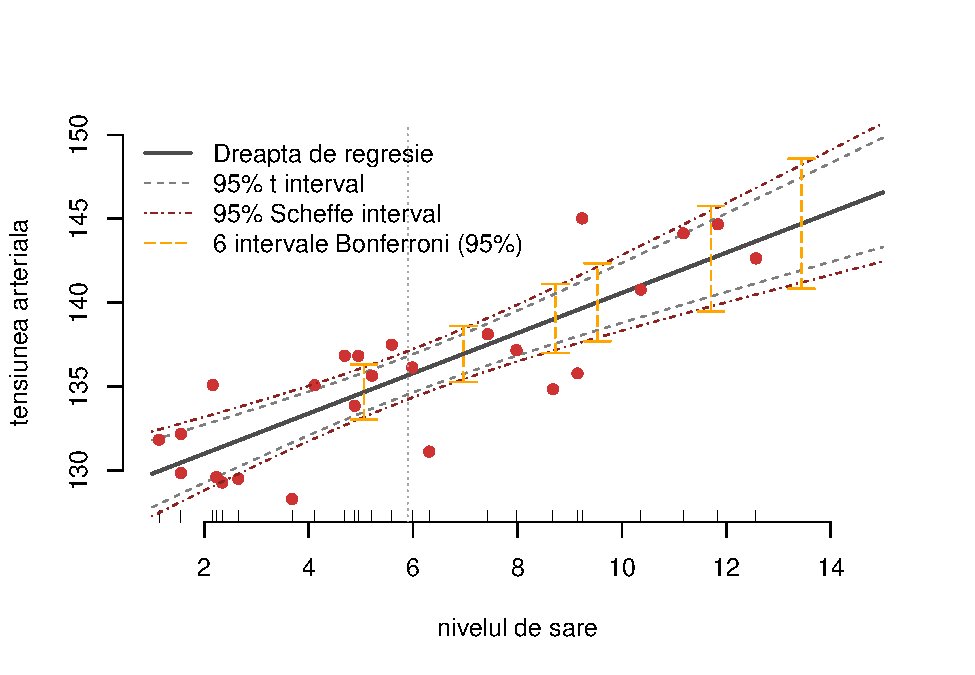
\includegraphics[width=0.8\linewidth]{Lab_6_files/figure-latex/unnamed-chunk-26-1} \end{center}

\subsubsection{Diagnostic}\label{diagnostic}

În această secțiune vom vedea dacă setul nostru de date verifică
ipotezele modelului de regresie liniară.

\begin{enumerate}
\def\labelenumi{\alph{enumi})}
\tightlist
\item
  \emph{Independența}
\end{enumerate}

Ipoteza de independență a variabilei răspuns (prin urmare și a erorilor)
reiese, de cele mai multe ori, din modalitatea în care s-a desfășurat
experimentul.

\begin{enumerate}
\def\labelenumi{\alph{enumi})}
\setcounter{enumi}{1}
\tightlist
\item
  \emph{Normalitatea}
\end{enumerate}

Pentru a verifica dacă ipoteza de normalitate a erorilor este
satisfăcută vom trasa dreapta lui Henry (sau Q-Q plot-ul):

\begin{Shaded}
\begin{Highlighting}[]
\CommentTok{# library(car)}
\KeywordTok{par}\NormalTok{(}\DataTypeTok{bty =} \StringTok{"n"}\NormalTok{)}
\KeywordTok{qqPlot}\NormalTok{(saltBP_model, }\DataTypeTok{col =} \StringTok{"brown3"}\NormalTok{, }\DataTypeTok{col.lines =} \StringTok{"grey50"}\NormalTok{, }\DataTypeTok{pch =} \DecValTok{16}\NormalTok{,}
       \DataTypeTok{simulate =} \OtherTok{TRUE}\NormalTok{,}
       \DataTypeTok{xlab =} \StringTok{"Cuantile teoretice"}\NormalTok{,}
       \DataTypeTok{ylab =} \StringTok{"Reziduuri studentizate"}\NormalTok{, }
       \DataTypeTok{main =} \StringTok{"Q-Q plot (Dreapta lui Henry)"}\NormalTok{,}
       \DataTypeTok{bty =} \StringTok{"n"}\NormalTok{)}
\end{Highlighting}
\end{Shaded}

\begin{center}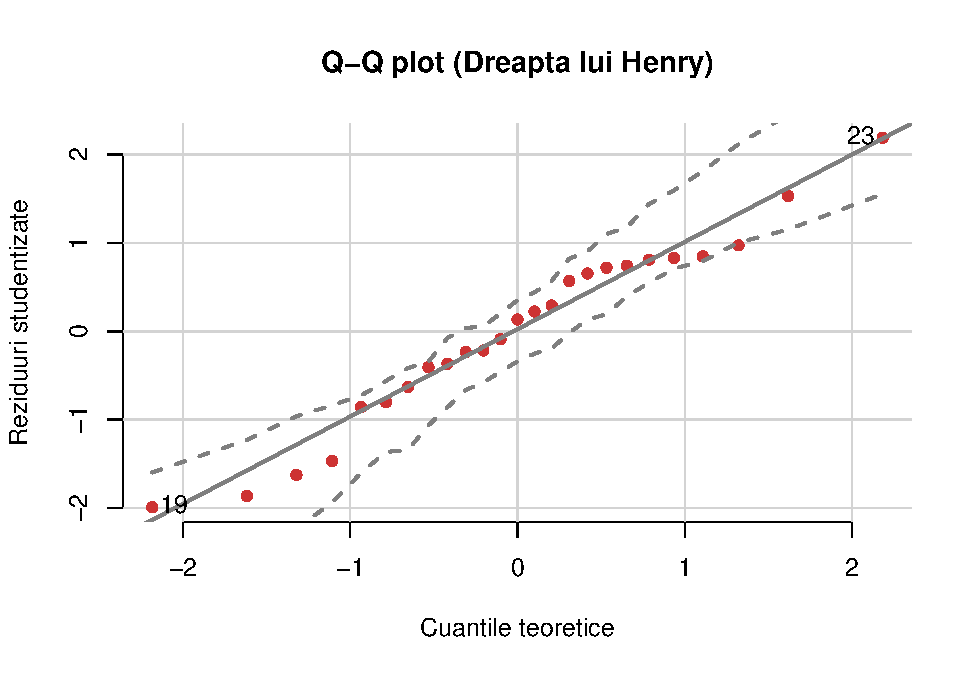
\includegraphics[width=0.8\linewidth]{Lab_6_files/figure-latex/unnamed-chunk-27-1} \end{center}

\begin{verbatim}
[1] 19 23
\end{verbatim}

Putem folosi și testul \texttt{Shapiro-Wilk}:

\begin{Shaded}
\begin{Highlighting}[]
\KeywordTok{shapiro.test}\NormalTok{(}\KeywordTok{residuals}\NormalTok{(saltBP_model))}

\NormalTok{    Shapiro}\OperatorTok{-}\NormalTok{Wilk normality test}

\NormalTok{data}\OperatorTok{:}\StringTok{  }\KeywordTok{residuals}\NormalTok{(saltBP_model)}
\NormalTok{W =}\StringTok{ }\FloatTok{0.96871}\NormalTok{, p}\OperatorTok{-}\NormalTok{value =}\StringTok{ }\FloatTok{0.6125}
\end{Highlighting}
\end{Shaded}

\begin{enumerate}
\def\labelenumi{\alph{enumi})}
\setcounter{enumi}{2}
\tightlist
\item
  \emph{Homoscedasticitatea}
\end{enumerate}

Pentru a verifica proprietatea de homoscedasticitate a erorilor vom
trasa un grafic al reziduurilor versus valorile prezise (fitted), i.e.
\(\hat{\varepsilon}\) vs \(\hat{y}\). Dacă avem homoscedasticitate a
erorilor atunci ar trebui să vedem o variație constantă pe verticală
(\(\hat{\varepsilon}\)).

\begin{Shaded}
\begin{Highlighting}[]
\KeywordTok{plot}\NormalTok{(}\KeywordTok{residuals}\NormalTok{(saltBP_model)}\OperatorTok{~}\KeywordTok{fitted}\NormalTok{(saltBP_model),  }\DataTypeTok{col =} \StringTok{"brown3"}\NormalTok{, }\DataTypeTok{pch =} \DecValTok{16}\NormalTok{, }
     \DataTypeTok{xlab =} \StringTok{"Valori prezise (fitted)"}\NormalTok{,}
     \DataTypeTok{ylab =} \StringTok{"Reziduuri"}\NormalTok{, }
     \DataTypeTok{main =} \StringTok{"Reziduuri vs Valori prezise"}\NormalTok{,}
     \DataTypeTok{bty =} \StringTok{"n"}\NormalTok{)}

\KeywordTok{abline}\NormalTok{(}\DataTypeTok{h =} \DecValTok{0}\NormalTok{, }\DataTypeTok{col =} \StringTok{"grey30"}\NormalTok{)}
\end{Highlighting}
\end{Shaded}

\begin{center}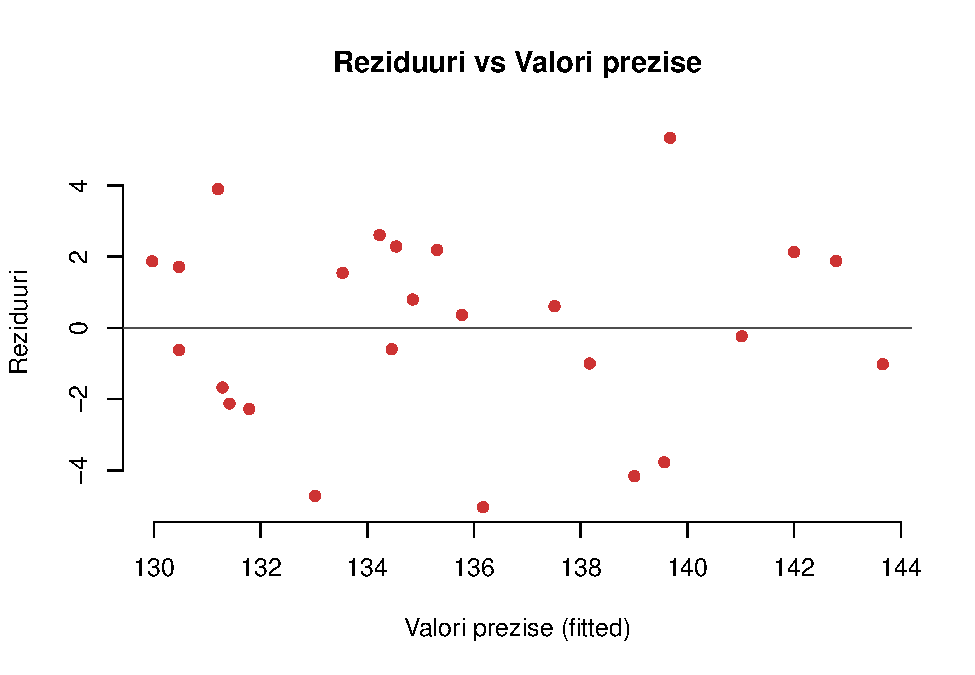
\includegraphics[width=0.8\linewidth]{Lab_6_files/figure-latex/unnamed-chunk-30-1} \end{center}

Tot în acest grafic putem observa dacă ipoteza de liniaritate este
verificată (în caz de liniaritate între variabila răspuns și variabila
cauză nu are trebui să vedem o relație sistematică între reziduuri și
valorile prezise - ceea ce se și întâmplă în cazul nostru) ori dacă
există o altă legătură structurală între variabila dependentă (răspuns)
și cea independentă (predictor).

\section{Regresie liniară multiplă}\label{regresie-liniara-multipla}

Modelul de regresie liniară multiplă reprezintă o generalizare a
modelului de regresie simplă. Dacă în regresia liniară simplă se folosea
o singură variabilă predictor \(X\) ca să explice variabila răspuns
\(Y\), în modelul de regresie liniară multiplă se folosesc mai multe
variabile predictor \(X_1,\ldots,X_k\) pentru a explica răspunsul \(Y\):

\[
\mathbb{E}[Y|X_1 = x_1, \ldots, X_k=x_x]=\beta_0+\beta_1x_1+\beta_2x_2+\ldots+\beta_kx_k
\] sau altfel scris

\[
Y = \beta_0 + \beta_1 X_1 + \ldots + \beta_k X_k + \varepsilon.
\]

Date fiind observațiile actuale, cu alte cuvinte dat fiind un eșantion
\((X_{11},\ldots,X_{1k},Y_1),\ldots,(X_{n1},\ldots,X_{nk},Y_n)\) al lui
\((X_1,\ldots,X_k,Y)\), unde \(X_{ij}\) reprezintă a \(i\)-a observație
a predictorului \(X_j\), modelul se poate scrie

\[
y_i = \beta_0+\beta_1x_{i1}+\beta_2x_{i2}+\ldots+\beta_kx_{ik}+\varepsilon_i, \quad i = 1,\ldots,n
\]

a cărui formă compactă (matriceală) este

\[
\mathbf{Y}=\mathbf{X}\boldsymbol\beta+\boldsymbol\varepsilon
\]

\begin{itemize}
\tightlist
\item
  \(\mathbf{X}\) este \emph{matricea de design}
\end{itemize}

\[
\mathbf{X}=\begin{pmatrix}
1 & X_{11} & \cdots & X_{1k}\\
\vdots & \vdots & \ddots & \vdots\\
1 & X_{n1} & \cdots & X_{nk}
\end{pmatrix}_{n\times(k+1)}
\]

\begin{itemize}
\tightlist
\item
  \(\mathbf{Y}\) este \emph{vectorul răspuns}, \(\boldsymbol\beta\) este
  \emph{vectorul coeficienților} iar \(\boldsymbol\varepsilon\) este
  \emph{vectorul eroare}
\end{itemize}

\[
\mathbf{Y}=\begin{pmatrix}
Y_1 \\
\vdots \\
Y_n
\end{pmatrix}_{n\times 1},\quad\boldsymbol\beta=\begin{pmatrix}
\beta_0 \\
\beta_1 \\
\vdots \\
\beta_k
\end{pmatrix}_{(k+1)\times 1}\text{ și }\quad
\boldsymbol\varepsilon=\begin{pmatrix}
\varepsilon_1 \\
\vdots \\
\varepsilon_n
\end{pmatrix}_{n\times 1}.
\]

\begin{rmdinsight}
Să observăm că pentru \(k=1\) modelul se reduce la regresia liniară
simplă. În acest caz:

\[
\mathbf{X}=\begin{pmatrix}
1 & X_{11}\\
\vdots & \vdots\\
1 & X_{n1}
\end{pmatrix}_{n\times2}\text{ și }\quad \beta=\begin{pmatrix}
\beta_0 \\
\beta_1 
\end{pmatrix}_{2\times 1}
\]
\end{rmdinsight}

\emph{Suma abaterilor pătratice reziduale} pentru modelul de regresie
liniară multiplă este

\[
RSS(\boldsymbol\beta)=\sum_{i=1}^n(Y_i-\beta_0-\beta_1X_{i1}-\ldots-\beta_kX_{ik})^2=(\mathbf{Y}-\mathbf{X}\boldsymbol{\beta})^T(\mathbf{Y}-\mathbf{X}\boldsymbol{\beta})
\]

ceea ce conduce la \emph{sistemul de ecuații normale}

\[
\mathbf{X}^\intercal\mathbf{X}\hat{\boldsymbol{\beta}}=\mathbf{X}^\intercal\mathbf{Y}
\]

a cărui soluție, dat fiind că \(\mathbf{X}^\intercal\mathbf{X}\) este
inversabilă, este

\[
\hat{\boldsymbol{\beta}}=(\mathbf{X}^\intercal\mathbf{X})^{-1}\mathbf{X}^\intercal\mathbf{Y}
\]

Odată ce avem estimatorul \(\hat{\boldsymbol{\beta}}\), putem defini:

\begin{itemize}
\tightlist
\item
  \emph{valorile prognozate} (\emph{fitted values})
  \(\hat Y_1,\ldots,\hat Y_n\) (valorile verticale pe hiperplanul de
  regresie), unde
\end{itemize}

\[
\hat Y_i=\hat\beta_0+\hat\beta_1X_{i1}+\cdots+\hat\beta_kX_{ik},\quad i=1,\ldots,n
\]

și sub formă matriceală

\[
\hat{\mathbf{Y}}=\mathbf{X}\hat{\boldsymbol{\beta}}=\mathbf{X}(\mathbf{X}^\intercal\mathbf{X})^{-1}\mathbf{X}^\intercal\mathbf{Y}=\mathbf{H}\mathbf{Y}
\]

unde
\(\mathbf{H}=\mathbf{X}(\mathbf{X}^\intercal\mathbf{X})^{-1}\mathbf{X}^\intercal\)
se numește \emph{matricea căciulă} (\emph{hat matrix}) și reprezintă
proiecția ortogonală a lui \(\mathbf{Y}\) în spațiul generat de
\(\mathbf{X}\).

\begin{itemize}
\tightlist
\item
  \emph{reziduurile estimate} (\emph{estimated residuals})
  \(\hat \varepsilon_1,\ldots,\hat \varepsilon_n\), unde
\end{itemize}

\[
\hat\varepsilon_i=Y_i-\hat Y_i,\quad i=1,\ldots,n
\]

și sub formă matriceală

\[
\hat{\boldsymbol\varepsilon} = \boldsymbol Y - \hat{\boldsymbol Y} = (\boldsymbol I-\boldsymbol H)\boldsymbol Y
\]

În figura de mai jos ilustrăm planul de regresie (albastru) și relația
cu regresiile liniare simple (liniile verzi). Punctele roșii reprezintă
un eșantion pentru \((X_1,X_2,Y)\) iar punctele negre sunt subeșantioane
pentru \((X_1,X_2)\) (la bază), \((X_1,Y)\) (stânga) și \((X_2,Y)\)
(dreapta).

\begin{center}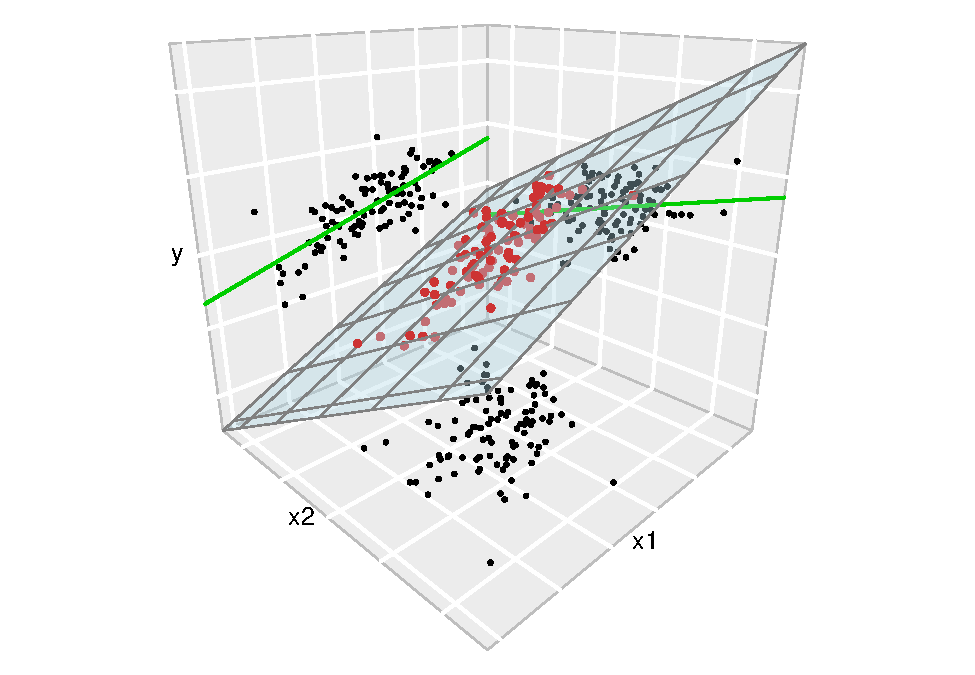
\includegraphics[width=0.8\linewidth]{Lab_6_files/figure-latex/unnamed-chunk-33-1} \end{center}

Ipotezele modelului sunt:

\begin{enumerate}
\def\labelenumi{\roman{enumi}.}
\tightlist
\item
  \textbf{Linearitatea}:
  \(\mathbb{E}[Y|X_1=x_1,\ldots,X_k=x_k]=\beta_0+\beta_1x_1+\ldots+\beta_kx_k\)
\item
  \textbf{Homoscedasticitatea}:
  \(\mathbb{V}\text{ar}(\varepsilon_i)=\sigma^2\), cu \(\sigma^2\)
  constantă pentru \(i=1,\ldots,n\)
\item
  \textbf{Normalitatea}: \(\varepsilon_i\sim\mathcal{N}(0,\sigma^2)\)
  pentru \(i=1,\ldots,n\)
\item
  \textbf{Independența erorilor}: \(\varepsilon_1,\ldots,\varepsilon_n\)
  sunt independente (sau necorelate,
  \(\mathbb{E}[\varepsilon_i\varepsilon_j]=0\), \(i\neq j\), deoarece
  sunt presupuse normale)
\end{enumerate}

Altfel spus

\[
Y|(X_1=x_1,\ldots,X_k=x_k)\sim \mathcal{N}(\beta_0+\beta_1x_1+\ldots+\beta_kx_k,\sigma^2)
\]

În figura de mai jos afișam planul de regresie. Spațiul dintre cele două
plane galbene arată unde se află 95\% din observații (după modelul
ales).

\begin{center}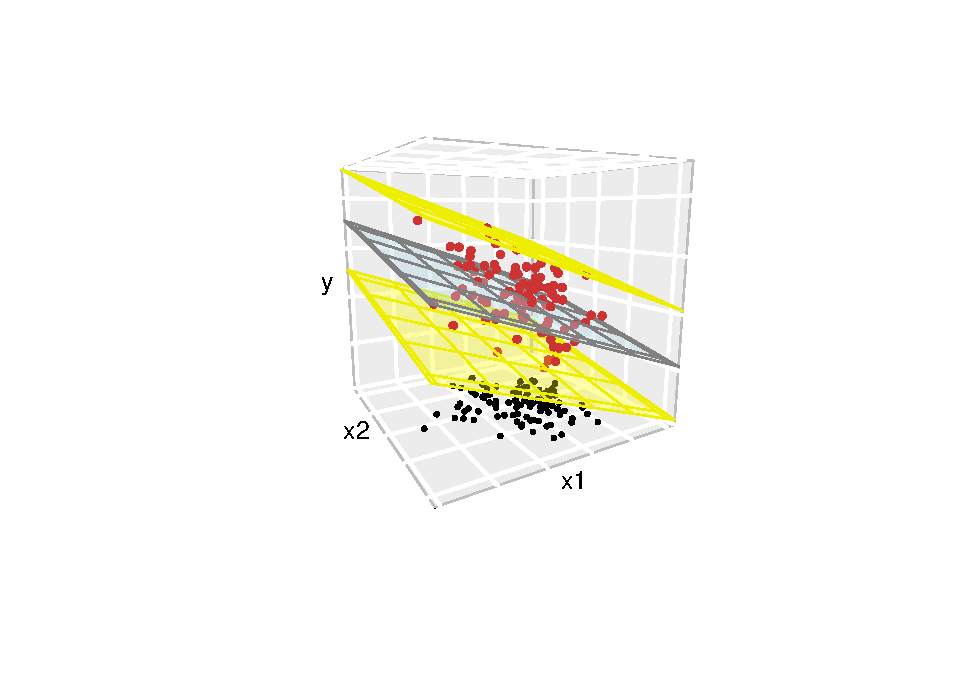
\includegraphics[width=0.8\linewidth]{Lab_6_files/figure-latex/unnamed-chunk-34-1} \end{center}

Estimatorul pentru \(\sigma^2\) este

\[
\hat{\sigma}^2 = \frac{RSS(\hat{\beta}_0,\hat{\beta}_1,\ldots, \hat{\beta}_k))}{n-(k+1)} = \frac{\hat{\boldsymbol \varepsilon}^\intercal\hat{\boldsymbol \varepsilon}}{n-(k+1)} = \frac{\sum_{i=1}^{n}\hat{\varepsilon}_i^2}{n-(k+1)}.
\]

\subsection{Aplicație}\label{aplicatie-1}

Această aplicație este bazată pe articolul \citep{Johnson1973}.

\begin{rmdexercise}
Considerăm setul de date \href{dataIn/galapagos.csv}{galapagos} care
conține informații despre numărul de specii de broaște țestoase din
diferite insule din arhipelagul Galapagos. Setul conține date din 30 de
insule despre numărul de specii de țestoase (\texttt{Species}), numărul
de specii endemice (\texttt{Endemics}), suprafața insulei
(\texttt{Area}), înălțimea maximă a insulei (`\texttt{Elevation}),
distanța la cea mai apropiată insulă (\texttt{Nearest}), distanța față
de insula Snata Cruz (\texttt{Scruz}) și suprafața insulei adiacente
(\texttt{Adjacent}). Vrem să investigăm relația liniară dintre numărul
de specii și celelalte variabile.
\end{rmdexercise}

Începem prin a citi datele

\begin{Shaded}
\begin{Highlighting}[]
\CommentTok{# gala = read.csv("data/galapagos.csv", row.names = 1)}

\KeywordTok{data}\NormalTok{(}\StringTok{"gala"}\NormalTok{) }\CommentTok{# este nevoie de libraria faraway}
\KeywordTok{head}\NormalTok{(gala)}
\NormalTok{             Species Endemics  Area Elevation Nearest Scruz Adjacent}
\NormalTok{Baltra            }\DecValTok{58}       \DecValTok{23} \FloatTok{25.09}       \DecValTok{346}     \FloatTok{0.6}   \FloatTok{0.6}     \FloatTok{1.84}
\NormalTok{Bartolome         }\DecValTok{31}       \DecValTok{21}  \FloatTok{1.24}       \DecValTok{109}     \FloatTok{0.6}  \FloatTok{26.3}   \FloatTok{572.33}
\NormalTok{Caldwell           }\DecValTok{3}        \DecValTok{3}  \FloatTok{0.21}       \DecValTok{114}     \FloatTok{2.8}  \FloatTok{58.7}     \FloatTok{0.78}
\NormalTok{Champion          }\DecValTok{25}        \DecValTok{9}  \FloatTok{0.10}        \DecValTok{46}     \FloatTok{1.9}  \FloatTok{47.4}     \FloatTok{0.18}
\NormalTok{Coamano            }\DecValTok{2}        \DecValTok{1}  \FloatTok{0.05}        \DecValTok{77}     \FloatTok{1.9}   \FloatTok{1.9}   \FloatTok{903.82}
\NormalTok{Daphne.Major      }\DecValTok{18}       \DecValTok{11}  \FloatTok{0.34}       \DecValTok{119}     \FloatTok{8.0}   \FloatTok{8.0}     \FloatTok{1.84}
\end{Highlighting}
\end{Shaded}

Considerăm modelul de regresie liniară multiplă cu 5 predictori:

\begin{Shaded}
\begin{Highlighting}[]
\NormalTok{gala_model =}\StringTok{ }\KeywordTok{lm}\NormalTok{(Species }\OperatorTok{~}\StringTok{ }\NormalTok{Area }\OperatorTok{+}\StringTok{ }\NormalTok{Elevation }\OperatorTok{+}\StringTok{ }\NormalTok{Nearest }\OperatorTok{+}\StringTok{ }\NormalTok{Scruz }\OperatorTok{+}\StringTok{ }\NormalTok{Adjacent, }\DataTypeTok{data=}\NormalTok{gala)}

\NormalTok{gala_model_summary =}\StringTok{ }\KeywordTok{summary}\NormalTok{(gala_model)}
\NormalTok{gala_model_summary}

\NormalTok{Call}\OperatorTok{:}
\KeywordTok{lm}\NormalTok{(}\DataTypeTok{formula =}\NormalTok{ Species }\OperatorTok{~}\StringTok{ }\NormalTok{Area }\OperatorTok{+}\StringTok{ }\NormalTok{Elevation }\OperatorTok{+}\StringTok{ }\NormalTok{Nearest }\OperatorTok{+}\StringTok{ }\NormalTok{Scruz }\OperatorTok{+}\StringTok{ }\NormalTok{Adjacent, }
    \DataTypeTok{data =}\NormalTok{ gala)}

\NormalTok{Residuals}\OperatorTok{:}
\StringTok{     }\NormalTok{Min       1Q   Median       3Q      Max }
\OperatorTok{-}\FloatTok{111.679}  \OperatorTok{-}\FloatTok{34.898}   \OperatorTok{-}\FloatTok{7.862}   \FloatTok{33.460}  \FloatTok{182.584} 

\NormalTok{Coefficients}\OperatorTok{:}
\StringTok{             }\NormalTok{Estimate Std. Error t value }\KeywordTok{Pr}\NormalTok{(}\OperatorTok{>}\ErrorTok{|}\NormalTok{t}\OperatorTok{|}\NormalTok{)    }
\NormalTok{(Intercept)  }\FloatTok{7.068221}  \FloatTok{19.154198}   \FloatTok{0.369} \FloatTok{0.715351}    
\NormalTok{Area        }\OperatorTok{-}\FloatTok{0.023938}   \FloatTok{0.022422}  \OperatorTok{-}\FloatTok{1.068} \FloatTok{0.296318}    
\NormalTok{Elevation    }\FloatTok{0.319465}   \FloatTok{0.053663}   \FloatTok{5.953} \FloatTok{3.82e-06} \OperatorTok{**}\ErrorTok{*}
\NormalTok{Nearest      }\FloatTok{0.009144}   \FloatTok{1.054136}   \FloatTok{0.009} \FloatTok{0.993151}    
\NormalTok{Scruz       }\OperatorTok{-}\FloatTok{0.240524}   \FloatTok{0.215402}  \OperatorTok{-}\FloatTok{1.117} \FloatTok{0.275208}    
\NormalTok{Adjacent    }\OperatorTok{-}\FloatTok{0.074805}   \FloatTok{0.017700}  \OperatorTok{-}\FloatTok{4.226} \FloatTok{0.000297} \OperatorTok{**}\ErrorTok{*}
\OperatorTok{---}
\NormalTok{Signif. codes}\OperatorTok{:}\StringTok{  }\DecValTok{0} \StringTok{'***'} \FloatTok{0.001} \StringTok{'**'} \FloatTok{0.01} \StringTok{'*'} \FloatTok{0.05} \StringTok{'.'} \FloatTok{0.1} \StringTok{' '} \DecValTok{1}

\NormalTok{Residual standard error}\OperatorTok{:}\StringTok{ }\FloatTok{60.98}\NormalTok{ on }\DecValTok{24}\NormalTok{ degrees of freedom}
\NormalTok{Multiple R}\OperatorTok{-}\NormalTok{squared}\OperatorTok{:}\StringTok{  }\FloatTok{0.7658}\NormalTok{,    Adjusted R}\OperatorTok{-}\NormalTok{squared}\OperatorTok{:}\StringTok{  }\FloatTok{0.7171} 
\NormalTok{F}\OperatorTok{-}\NormalTok{statistic}\OperatorTok{:}\StringTok{  }\FloatTok{15.7}\NormalTok{ on }\DecValTok{5}\NormalTok{ and }\DecValTok{24}\NormalTok{ DF,  p}\OperatorTok{-}\NormalTok{value}\OperatorTok{:}\StringTok{ }\FloatTok{6.838e-07}
\end{Highlighting}
\end{Shaded}

\subsubsection{Estimarea parametrilor}\label{estimarea-parametrilor-1}

Pentru început extragem matricea de design \(X\)

\begin{Shaded}
\begin{Highlighting}[]
\NormalTok{X =}\StringTok{ }\KeywordTok{model.matrix}\NormalTok{( }\OperatorTok{~}\StringTok{ }\NormalTok{Area }\OperatorTok{+}\StringTok{ }\NormalTok{Elevation }\OperatorTok{+}\StringTok{ }\NormalTok{Nearest }\OperatorTok{+}\StringTok{ }\NormalTok{Scruz }\OperatorTok{+}\StringTok{ }\NormalTok{Adjacent, }
    \DataTypeTok{data =}\NormalTok{ gala)}

\KeywordTok{head}\NormalTok{(X)}
\NormalTok{             (Intercept)  Area Elevation Nearest Scruz Adjacent}
\NormalTok{Baltra                 }\DecValTok{1} \FloatTok{25.09}       \DecValTok{346}     \FloatTok{0.6}   \FloatTok{0.6}     \FloatTok{1.84}
\NormalTok{Bartolome              }\DecValTok{1}  \FloatTok{1.24}       \DecValTok{109}     \FloatTok{0.6}  \FloatTok{26.3}   \FloatTok{572.33}
\NormalTok{Caldwell               }\DecValTok{1}  \FloatTok{0.21}       \DecValTok{114}     \FloatTok{2.8}  \FloatTok{58.7}     \FloatTok{0.78}
\NormalTok{Champion               }\DecValTok{1}  \FloatTok{0.10}        \DecValTok{46}     \FloatTok{1.9}  \FloatTok{47.4}     \FloatTok{0.18}
\NormalTok{Coamano                }\DecValTok{1}  \FloatTok{0.05}        \DecValTok{77}     \FloatTok{1.9}   \FloatTok{1.9}   \FloatTok{903.82}
\NormalTok{Daphne.Major           }\DecValTok{1}  \FloatTok{0.34}       \DecValTok{119}     \FloatTok{8.0}   \FloatTok{8.0}     \FloatTok{1.84}
\end{Highlighting}
\end{Shaded}

și răspunsul \(y\)

\begin{Shaded}
\begin{Highlighting}[]
\NormalTok{y =}\StringTok{ }\NormalTok{gala}\OperatorTok{$}\NormalTok{Species}
\end{Highlighting}
\end{Shaded}

Vrem să găsim
\(\hat{\boldsymbol{\beta}}=(\mathbf{X}^\intercal\mathbf{X})^{-1}\mathbf{X}^\intercal\mathbf{Y}\)

\begin{Shaded}
\begin{Highlighting}[]
\CommentTok{# determinam (\textbackslash{}mathbf\{X\}^\textbackslash{}intercal\textbackslash{}mathbf\{X\})^\{-1\}}

\NormalTok{xtxi =}\StringTok{ }\KeywordTok{solve}\NormalTok{(}\KeywordTok{t}\NormalTok{(X) }\OperatorTok\StringTok{ }\NormalTok{X) }\CommentTok{# t() - este transpusa}
                         \CommentTok{# %*% - produsul matriceal}
                         \CommentTok{# solve() - calculeaza pseudoinversa}

\NormalTok{bHat =}\StringTok{ }\NormalTok{xtxi }\OperatorTok\StringTok{ }\KeywordTok{t}\NormalTok{(X) }\OperatorTok\StringTok{ }\NormalTok{y}
\NormalTok{bHat}
\NormalTok{                    [,}\DecValTok{1}\NormalTok{]}
\NormalTok{(Intercept)  }\FloatTok{7.068220709}
\NormalTok{Area        }\OperatorTok{-}\FloatTok{0.023938338}
\NormalTok{Elevation    }\FloatTok{0.319464761}
\NormalTok{Nearest      }\FloatTok{0.009143961}
\NormalTok{Scruz       }\OperatorTok{-}\FloatTok{0.240524230}
\NormalTok{Adjacent    }\OperatorTok{-}\FloatTok{0.074804832}
\end{Highlighting}
\end{Shaded}

sau alternativ folosind ecuațiile normalw

\begin{Shaded}
\begin{Highlighting}[]
\KeywordTok{solve}\NormalTok{(}\KeywordTok{crossprod}\NormalTok{(X,X), }\KeywordTok{crossprod}\NormalTok{(X,y)) }\CommentTok{# crossprod calculeaza X^Ty}
\NormalTok{                    [,}\DecValTok{1}\NormalTok{]}
\NormalTok{(Intercept)  }\FloatTok{7.068220709}
\NormalTok{Area        }\OperatorTok{-}\FloatTok{0.023938338}
\NormalTok{Elevation    }\FloatTok{0.319464761}
\NormalTok{Nearest      }\FloatTok{0.009143961}
\NormalTok{Scruz       }\OperatorTok{-}\FloatTok{0.240524230}
\NormalTok{Adjacent    }\OperatorTok{-}\FloatTok{0.074804832}
\end{Highlighting}
\end{Shaded}

Estimatorul pentru \(\sigma^2\) este dat de

\begin{Shaded}
\begin{Highlighting}[]
\NormalTok{sHat =}\StringTok{ }\KeywordTok{sqrt}\NormalTok{(}\KeywordTok{deviance}\NormalTok{(gala_model)}\OperatorTok{/}\KeywordTok{df.residual}\NormalTok{(gala_model))}
\NormalTok{sHat}
\NormalTok{[}\DecValTok{1}\NormalTok{] }\FloatTok{60.97519}
\end{Highlighting}
\end{Shaded}

sau încă de

\begin{Shaded}
\begin{Highlighting}[]
\NormalTok{gala_model_summary}\OperatorTok{$}\NormalTok{sigma}
\NormalTok{[}\DecValTok{1}\NormalTok{] }\FloatTok{60.97519}
\end{Highlighting}
\end{Shaded}

Dacă vrem să determinăm erorile standard ale coeficienților, i.e.
\(\hat{\mathrm{SE}}(\hat\beta_i)\), să observăm pentru început că
acestea sunt date de următoarea formulă

\[
\hat{\mathrm{SE}}(\hat\beta_{i-1}) = \hat{\sigma}\sqrt{(\mathbf{X}^\intercal\mathbf{X})^{-1}_{ii}}
\]

unde \((\mathbf{X}^\intercal\mathbf{X})^{-1}_{ii}\) reprezintă elementul
\(i\) de pe diagonala matricii
\((\mathbf{X}^\intercal\mathbf{X})^{-1}\). Avem

\begin{Shaded}
\begin{Highlighting}[]
\NormalTok{seBHat =}\StringTok{ }\NormalTok{sHat}\OperatorTok{*}\KeywordTok{sqrt}\NormalTok{(}\KeywordTok{diag}\NormalTok{(xtxi))}
\NormalTok{seBHat}
\NormalTok{(Intercept)        Area   Elevation     Nearest       Scruz    Adjacent }
\FloatTok{19.15419782}  \FloatTok{0.02242235}  \FloatTok{0.05366280}  \FloatTok{1.05413595}  \FloatTok{0.21540225}  \FloatTok{0.01770019} 
\end{Highlighting}
\end{Shaded}

sau folosind modelul sumarizat

\begin{Shaded}
\begin{Highlighting}[]
\NormalTok{gala_model_summary}\OperatorTok{$}\NormalTok{coefficients[, }\DecValTok{2}\NormalTok{]}
\NormalTok{(Intercept)        Area   Elevation     Nearest       Scruz    Adjacent }
\FloatTok{19.15419782}  \FloatTok{0.02242235}  \FloatTok{0.05366280}  \FloatTok{1.05413595}  \FloatTok{0.21540225}  \FloatTok{0.01770019} 
\end{Highlighting}
\end{Shaded}

\subsubsection{Inferență asupra
parametrilor}\label{inferenta-asupra-parametrilor-1}

Având mai mulți predictori pentru o variabilă răspuns, ne întrebăm dacă
avem nevoie de toți. Fie \(\Theta\) spațiul parametrilor pentru un model
mai mare și \(\Theta_0\) spațiul parametrilor pentru un model mai mic
(\(\Theta_0\subset \Theta\)). Dacă nu avem o diferență prea mare între
concordanța celor două modele atunci îl preferăm pe cel mai simplu.
Testul bazat pe raportul de verosimilități (\(H_0: \theta\in \Theta_0\)
vs \(H_1: \theta\in\Theta\)) conduce la respingerea ipotezei nule în
cazul în care raportul

\[
\frac{RSS_{\Theta_0}-RSS_{\Theta}}{RSS_{\Theta}}
\]

este suficient de mare. Dacă spațiul parametrilor \(\Theta\) are
dimensiunea \(p\) (la noi \(k+1\)) iar spațiul parametrilor modelului
redus \(\Theta_0\) are dimensiunea \(q\) atunci

\[
F = \frac{\frac{RSS_{\Theta_0}-RSS_{\Theta}}{(p-q)}}{\frac{RSS_{\Theta}}{n-p}} = \frac{\frac{RSS_{\Theta_0}-RSS_{\Theta}}{(df_{\Theta_0}-df_{\Theta})}}{\frac{RSS_{\Theta}}{df_{\Theta}}} \sim F_{p-q,n-p}.
\]

unde \(df_{\Theta_0}=n-q\) iar \(df_{\Theta} = n-p\) (gradele de
libertate sunt în general numărul de observații minus numărul de
parametrii ai modelului).

\begin{enumerate}
\def\labelenumi{\alph{enumi})}
\tightlist
\item
  Test asupra tuturor predictorilor
\end{enumerate}

Să presupunem că vrem să testăm ipoteza nulă

\[
H_0: \beta_1 = \cdots = \beta_k = 0
\]

cu alte cuvinte vrem să răspundem la întrebarea dacă vreuna din
variabilele explicative este folositoare în prezicerea răspunsului. În
această situație modelul (complet \(\Theta\)) este
\(\boldsymbol y = \boldsymbol X\boldsymbol \beta+\boldsymbol\varepsilon\)
și are \(k+1\) parametrii (\(k+1\) coeficienți \(\beta_i\)) iar modelul
redus (\(\Theta_0\)) este
\(\boldsymbol y = \boldsymbol \mu+\boldsymbol\varepsilon\) și are \(1\)
parametru (\(\beta_0\)). Prin urmare avem statistica \(F\)

\[
F = \frac{\frac{RSS_{\Theta_0}-RSS_{\Theta}}{(k+1-1)}}{\frac{RSS_{\Theta}}{n-(k+1)}} = \frac{\frac{SS_{T}-RSS}{k}}{\frac{RSS}{n-(k+1)}}= \frac{\frac{SS_{reg}}{k}}{\frac{RSS}{n-(k+1)}}\sim F_{k,n-(k+1)}
\]

unde \(RSS\) este suma abaterilor pătratice reziduale,
\(SS_T=(\boldsymbol y - \bar{\boldsymbol y})^\intercal(\boldsymbol y - \bar{\boldsymbol y})\)
este suma abaterilor pătratice totale iar \(SS_{reg}=SS_{T}-RSS\) este
suma abaterilor de regresie, ceea ce conduce la tabelul ANOVA

\begin{longtable}[]{@{}llllll@{}}
\toprule
& Df & SS & MS & \(F\) & \(p\)-value\tabularnewline
\midrule
\endhead
Regresie & \(k\) & \(SS_{reg}\) & \(\frac{SS_{reg}}{k}\) &
\(F=\frac{SS_{reg}/k}{RSS/(n-(k+1))}\) & \(p\)\tabularnewline
Residuuri & \(n - (k+1)\) & \(RSS\) & \(\frac{RSS}{n-(k+1)}\) &
&\tabularnewline
Total & \(n-1\) & \(SS_{T}\) & & &\tabularnewline
\bottomrule
\end{longtable}

Chiar dacă ipoteza nulă a fost respinsă asta nu înseamnă că modelul dat
de alternativă este cel mai bun (nu știm dacă toți predictorii sunt
necesari în model sau doar o parte dintre ei).

Pentru setul nostru de date să considerăm modelul nul (cel ce corespunde
lui \(\Theta_0\))

\begin{Shaded}
\begin{Highlighting}[]
\NormalTok{gala_null_model =}\StringTok{ }\KeywordTok{lm}\NormalTok{(Species }\OperatorTok{~}\StringTok{ }\DecValTok{1}\NormalTok{, }\DataTypeTok{data =}\NormalTok{ gala)}
\end{Highlighting}
\end{Shaded}

Tabelul ANOVA este dat de

\begin{Shaded}
\begin{Highlighting}[]
\KeywordTok{anova}\NormalTok{(gala_model, gala_null_model)}
\NormalTok{Analysis of Variance Table}

\NormalTok{Model }\DecValTok{1}\OperatorTok{:}\StringTok{ }\NormalTok{Species }\OperatorTok{~}\StringTok{ }\NormalTok{Area }\OperatorTok{+}\StringTok{ }\NormalTok{Elevation }\OperatorTok{+}\StringTok{ }\NormalTok{Nearest }\OperatorTok{+}\StringTok{ }\NormalTok{Scruz }\OperatorTok{+}\StringTok{ }\NormalTok{Adjacent}
\NormalTok{Model }\DecValTok{2}\OperatorTok{:}\StringTok{ }\NormalTok{Species }\OperatorTok{~}\StringTok{ }\DecValTok{1}
\NormalTok{  Res.Df    RSS Df Sum of Sq      F    }\KeywordTok{Pr}\NormalTok{(}\OperatorTok{>}\NormalTok{F)    }
\DecValTok{1}     \DecValTok{24}  \DecValTok{89231}                                  
\DecValTok{2}     \DecValTok{29} \DecValTok{381081} \OperatorTok{-}\DecValTok{5}   \OperatorTok{-}\DecValTok{291850} \FloatTok{15.699} \FloatTok{6.838e-07} \OperatorTok{**}\ErrorTok{*}
\OperatorTok{---}
\NormalTok{Signif. codes}\OperatorTok{:}\StringTok{  }\DecValTok{0} \StringTok{'***'} \FloatTok{0.001} \StringTok{'**'} \FloatTok{0.01} \StringTok{'*'} \FloatTok{0.05} \StringTok{'.'} \FloatTok{0.1} \StringTok{' '} \DecValTok{1}
\end{Highlighting}
\end{Shaded}

Observăm că ipoteza nulă este respinsă în acest caz în favoarea
alternativei (p valoarea este aproximativ \(6.8\times 10^{-7}\)).

Putem calcula această p-valoare și fără a apela la ajutorul funcției
\texttt{anova}:

\begin{Shaded}
\begin{Highlighting}[]
\CommentTok{# pentru modelul redus }
\NormalTok{RSS0 =}\StringTok{ }\KeywordTok{deviance}\NormalTok{(gala_null_model)}
\NormalTok{df0 =}\StringTok{ }\KeywordTok{df.residual}\NormalTok{(gala_null_model)}

\CommentTok{# pentru modelul intreg}
\NormalTok{RSS =}\StringTok{ }\KeywordTok{deviance}\NormalTok{(gala_model)}
\NormalTok{df =}\StringTok{ }\KeywordTok{df.residual}\NormalTok{(gala_model)}

\CommentTok{# statistica F}

\NormalTok{Fstat =}\StringTok{ }\NormalTok{((RSS0 }\OperatorTok{-}\StringTok{ }\NormalTok{RSS)}\OperatorTok{/}\NormalTok{(df0 }\OperatorTok{-}\StringTok{ }\NormalTok{df))}\OperatorTok{/}\NormalTok{(RSS}\OperatorTok{/}\NormalTok{df)}

\DecValTok{1}\OperatorTok{-}\KeywordTok{pf}\NormalTok{(Fstat, df0}\OperatorTok{-}\NormalTok{df, df)}
\NormalTok{[}\DecValTok{1}\NormalTok{] }\FloatTok{6.837893e-07}
\end{Highlighting}
\end{Shaded}

\begin{enumerate}
\def\labelenumi{\alph{enumi})}
\setcounter{enumi}{1}
\tightlist
\item
  Test asupra unui predictor
\end{enumerate}

Să presupunem acum că vrem să testăm dacă putem exclude din model un
anumit predictor \(i\) (fixat). Prin urmare vrem să testăm ipoteza nulă

\[
H_0:\beta_i=0
\]

Considerăm modelul întreg \(\Theta\) în care avem toți predictorii și
modelul redus \(\Theta_0\) în care avem toți predictorii mai puțin
predictorul \(i\) (în cazul problemei noastre o să testăm să vedem dacă
putem exclude sau nu variabila explicativă \texttt{Area}):

\begin{Shaded}
\begin{Highlighting}[]
\NormalTok{gala_Area_model =}\StringTok{ }\KeywordTok{lm}\NormalTok{(Species }\OperatorTok{~}\StringTok{ }\NormalTok{Elevation }\OperatorTok{+}\StringTok{ }\NormalTok{Nearest }\OperatorTok{+}\StringTok{ }\NormalTok{Scruz }\OperatorTok{+}\StringTok{ }\NormalTok{Adjacent, }
    \DataTypeTok{data =}\NormalTok{ gala)}

\KeywordTok{anova}\NormalTok{(gala_model, gala_Area_model)}
\NormalTok{Analysis of Variance Table}

\NormalTok{Model }\DecValTok{1}\OperatorTok{:}\StringTok{ }\NormalTok{Species }\OperatorTok{~}\StringTok{ }\NormalTok{Area }\OperatorTok{+}\StringTok{ }\NormalTok{Elevation }\OperatorTok{+}\StringTok{ }\NormalTok{Nearest }\OperatorTok{+}\StringTok{ }\NormalTok{Scruz }\OperatorTok{+}\StringTok{ }\NormalTok{Adjacent}
\NormalTok{Model }\DecValTok{2}\OperatorTok{:}\StringTok{ }\NormalTok{Species }\OperatorTok{~}\StringTok{ }\NormalTok{Elevation }\OperatorTok{+}\StringTok{ }\NormalTok{Nearest }\OperatorTok{+}\StringTok{ }\NormalTok{Scruz }\OperatorTok{+}\StringTok{ }\NormalTok{Adjacent}
\NormalTok{  Res.Df   RSS Df Sum of Sq      F }\KeywordTok{Pr}\NormalTok{(}\OperatorTok{>}\NormalTok{F)}
\DecValTok{1}     \DecValTok{24} \DecValTok{89231}                           
\DecValTok{2}     \DecValTok{25} \DecValTok{93469} \OperatorTok{-}\DecValTok{1}   \OperatorTok{-}\FloatTok{4237.7} \FloatTok{1.1398} \FloatTok{0.2963}
\end{Highlighting}
\end{Shaded}

Observăm că nu putem respinge ipoteza nulă (p valoarea \(>0.05\)).

O abordare alternativă constă în folosirea statisticii de test

\[
t_i = \frac{\hat\beta_i}{\hat{\mathrm{SE}}(\hat\beta_j)}\sim_{H_0} t_{n-k-1}
\]

care verifică relația \(t_i^2 = F\). Putem vedea statistica student în
output-ul funcției \texttt{summary}:

\begin{Shaded}
\begin{Highlighting}[]
\NormalTok{gala_model_summary}\OperatorTok{$}\NormalTok{coefficients}
\NormalTok{                Estimate  Std. Error      t value     }\KeywordTok{Pr}\NormalTok{(}\OperatorTok{>}\ErrorTok{|}\NormalTok{t}\OperatorTok{|}\NormalTok{)}
\NormalTok{(Intercept)  }\FloatTok{7.068220709} \FloatTok{19.15419782}  \FloatTok{0.369016796} \FloatTok{7.153508e-01}
\NormalTok{Area        }\OperatorTok{-}\FloatTok{0.023938338}  \FloatTok{0.02242235} \OperatorTok{-}\FloatTok{1.067610554} \FloatTok{2.963180e-01}
\NormalTok{Elevation    }\FloatTok{0.319464761}  \FloatTok{0.05366280}  \FloatTok{5.953187968} \FloatTok{3.823409e-06}
\NormalTok{Nearest      }\FloatTok{0.009143961}  \FloatTok{1.05413595}  \FloatTok{0.008674366} \FloatTok{9.931506e-01}
\NormalTok{Scruz       }\OperatorTok{-}\FloatTok{0.240524230}  \FloatTok{0.21540225} \OperatorTok{-}\FloatTok{1.116628222} \FloatTok{2.752082e-01}
\NormalTok{Adjacent    }\OperatorTok{-}\FloatTok{0.074804832}  \FloatTok{0.01770019} \OperatorTok{-}\FloatTok{4.226216850} \FloatTok{2.970655e-04}
\end{Highlighting}
\end{Shaded}

\begin{enumerate}
\def\labelenumi{\alph{enumi})}
\setcounter{enumi}{2}
\tightlist
\item
  Test pentru o pereche de predictori
\end{enumerate}

Să presupunem că vrem să testăm dacă suprafața insulei curente sau a
insulei adiacente au vreo relație relativ la variabila răspuns. Prin
urmare vrem să testăm ipoteza nulă (\textbf{să ținem cont că trebuie să
specificăm care sunt toți predictorii !})

\[
H_0:\beta_i=\beta_j=0\quad(\beta_{Area}=\beta_{Adjacent}=0)
\]

Putem testa această ipoteză folosind procedura descrisă anterior:

\begin{Shaded}
\begin{Highlighting}[]
\NormalTok{gala_Area_Adjacent_model =}\StringTok{ }\KeywordTok{lm}\NormalTok{(Species }\OperatorTok{~}\StringTok{ }\NormalTok{Elevation }\OperatorTok{+}\StringTok{ }\NormalTok{Nearest }\OperatorTok{+}\StringTok{ }\NormalTok{Scruz, }
    \DataTypeTok{data =}\NormalTok{ gala)}

\KeywordTok{anova}\NormalTok{(gala_Area_Adjacent_model, gala_model)}
\NormalTok{Analysis of Variance Table}

\NormalTok{Model }\DecValTok{1}\OperatorTok{:}\StringTok{ }\NormalTok{Species }\OperatorTok{~}\StringTok{ }\NormalTok{Elevation }\OperatorTok{+}\StringTok{ }\NormalTok{Nearest }\OperatorTok{+}\StringTok{ }\NormalTok{Scruz}
\NormalTok{Model }\DecValTok{2}\OperatorTok{:}\StringTok{ }\NormalTok{Species }\OperatorTok{~}\StringTok{ }\NormalTok{Area }\OperatorTok{+}\StringTok{ }\NormalTok{Elevation }\OperatorTok{+}\StringTok{ }\NormalTok{Nearest }\OperatorTok{+}\StringTok{ }\NormalTok{Scruz }\OperatorTok{+}\StringTok{ }\NormalTok{Adjacent}
\NormalTok{  Res.Df    RSS Df Sum of Sq      F  }\KeywordTok{Pr}\NormalTok{(}\OperatorTok{>}\NormalTok{F)   }
\DecValTok{1}     \DecValTok{26} \DecValTok{158292}                               
\DecValTok{2}     \DecValTok{24}  \DecValTok{89231}  \DecValTok{2}     \DecValTok{69060} \FloatTok{9.2874} \FloatTok{0.00103} \OperatorTok{**}
\OperatorTok{---}
\NormalTok{Signif. codes}\OperatorTok{:}\StringTok{  }\DecValTok{0} \StringTok{'***'} \FloatTok{0.001} \StringTok{'**'} \FloatTok{0.01} \StringTok{'*'} \FloatTok{0.05} \StringTok{'.'} \FloatTok{0.1} \StringTok{' '} \DecValTok{1}
\end{Highlighting}
\end{Shaded}

Observăm că ipoteza nulă este respinsă deoarece p-valoarea este mică
(prin urmare excluderea celor doi predictori nu este justificată).

\subsubsection{Intervale de încredere pentru
parametrii}\label{intervale-de-incredere-pentru-parametrii-1}

Cum repartiția lui \(\hat{\boldsymbol{\beta}}\) este:

\[
\hat{\boldsymbol{\beta}}\sim\mathcal{N}_{k+1}\left(\boldsymbol\beta,\sigma^2(\mathbf{X}^T\mathbf{X})^{-1}\right)
\]

atunci estimatorul \(\hat\sigma^2\) pentru \(\sigma^2\) obținem că

\[
\frac{\hat\beta_j-\beta_j}{\hat{\mathrm{SE}}(\hat\beta_j)}\sim t_{n-(k+1)}
\]

iar un interval de încredere de nivel \(1-\alpha\) pentru parametrul
\(\beta_j\) este

\[
IC = \left(\hat\beta_j\pm\hat{\mathrm{SE}}(\hat\beta_j)t_{n-2;1-\alpha/2}\right)
\]

Putem construi intervale de încredere pentru parametrii folosind funcția
\texttt{confint}:

\begin{Shaded}
\begin{Highlighting}[]
\KeywordTok{confint}\NormalTok{(gala_model)}
                  \FloatTok{2.5} \OperatorTok
\NormalTok{(Intercept) }\OperatorTok{-}\FloatTok{32.4641006} \FloatTok{46.60054205}
\NormalTok{Area         }\OperatorTok{-}\FloatTok{0.0702158}  \FloatTok{0.02233912}
\NormalTok{Elevation     }\FloatTok{0.2087102}  \FloatTok{0.43021935}
\NormalTok{Nearest      }\OperatorTok{-}\FloatTok{2.1664857}  \FloatTok{2.18477363}
\NormalTok{Scruz        }\OperatorTok{-}\FloatTok{0.6850926}  \FloatTok{0.20404416}
\NormalTok{Adjacent     }\OperatorTok{-}\FloatTok{0.1113362} \OperatorTok{-}\FloatTok{0.03827344}
\end{Highlighting}
\end{Shaded}

Dacă vrem să construim o regiune de încredere pentru mai mult de un
parametru atunci putem să folosim relația:

\[
(\hat{\boldsymbol \beta} - \boldsymbol \beta)^\intercal\boldsymbol X^\intercal \boldsymbol X (\hat{\boldsymbol \beta} - \boldsymbol \beta)\leq (k+1)\hat{\boldsymbol \sigma}^2F_{k+1, n-(k+1)}^{1-\alpha}
\]

care reprezintă o regiune de încredere pentru \(\boldsymbol \beta\).

De exemplu vrem să construim o regiune de încredere pentru perechea
\((\beta_{Area},\beta_{Adjacent})\):

\begin{Shaded}
\begin{Highlighting}[]
\KeywordTok{par}\NormalTok{(}\DataTypeTok{bty =} \StringTok{"n"}\NormalTok{)}
\KeywordTok{confidenceEllipse}\NormalTok{(gala_model, }\DataTypeTok{which.coef =} \KeywordTok{c}\NormalTok{(}\DecValTok{2}\NormalTok{,}\DecValTok{6}\NormalTok{),}
                  \DataTypeTok{xlab =} \StringTok{"Area"}\NormalTok{, }
                  \DataTypeTok{ylab =} \StringTok{"Adjacent"}\NormalTok{,}
                  \DataTypeTok{col =} \StringTok{"grey30"}\NormalTok{,}
                  \DataTypeTok{ylim =} \KeywordTok{c}\NormalTok{(}\OperatorTok{-}\FloatTok{0.15}\NormalTok{,}\FloatTok{0.005}\NormalTok{)) }
\KeywordTok{points}\NormalTok{(}\DecValTok{0}\NormalTok{, }\DecValTok{0}\NormalTok{, }\DataTypeTok{pch =} \DecValTok{18}\NormalTok{, }\DataTypeTok{col =} \StringTok{"brown3"}\NormalTok{,}
       \DataTypeTok{cex =} \DecValTok{2}\NormalTok{)}
\KeywordTok{abline}\NormalTok{(}\DataTypeTok{v =} \KeywordTok{confint}\NormalTok{(gala_model)[}\DecValTok{2}\NormalTok{,], }\DataTypeTok{lty =} \DecValTok{2}\NormalTok{)}
\KeywordTok{abline}\NormalTok{(}\DataTypeTok{h =} \KeywordTok{confint}\NormalTok{(gala_model)[}\DecValTok{6}\NormalTok{,], }\DataTypeTok{lty =} \DecValTok{2}\NormalTok{)}
\end{Highlighting}
\end{Shaded}

\begin{center}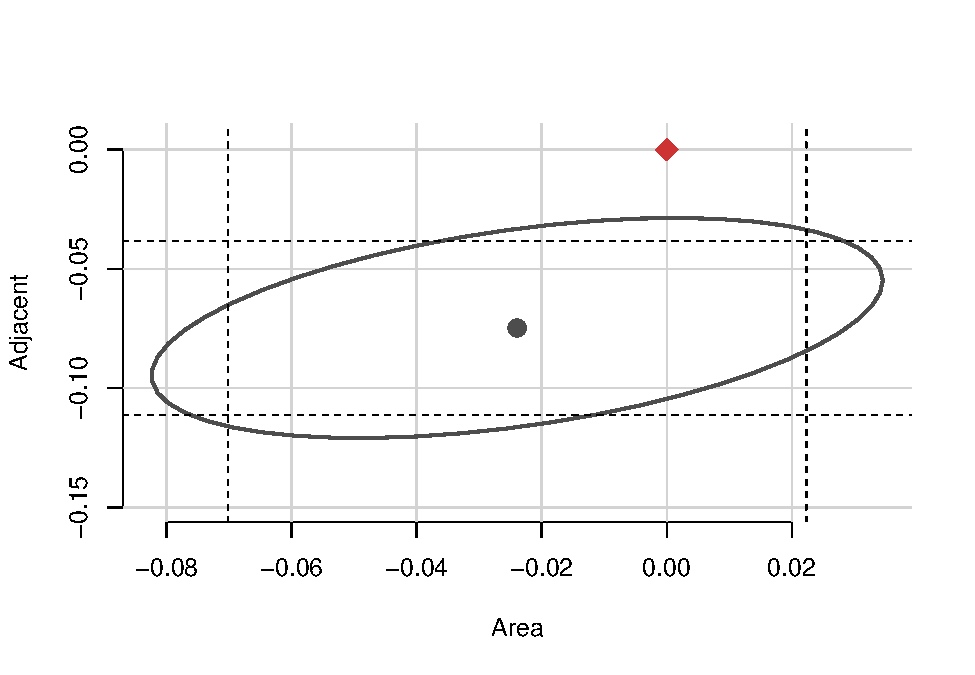
\includegraphics[width=0.8\linewidth]{Lab_6_files/figure-latex/unnamed-chunk-53-1} \end{center}

Cum punctul \((0,0)\) nu aparține regiunii elipsoidale atunci putem
respinge ipoteza nulă \(H_0:\beta_{Area}=\beta_{Adjacent}=0\).

\renewcommand\refname{Referințe}
\bibliography{references/Biostat2018ref.bib}


\end{document}
